\documentclass[11pt, a4paper,svglistings]{report}
\usepackage{a4wide}
\usepackage[USenglish]{babel}
\usepackage{graphicx}
\usepackage{float}
\usepackage{mathtools}

\setcounter{secnumdepth}{5}   
\setcounter{tocdepth}{5}   

\usepackage[toc,page]{appendix}

\usepackage{hyperref}
\hypersetup{
    colorlinks,
    citecolor=black,
    filecolor=black,
    linkcolor=black,
    urlcolor=black
}

\usepackage{fullpage}
\usepackage{listings}
\usepackage{xcolor}
\usepackage{textcomp}

\usepackage[explicit]{titlesec}
\usepackage{lmodern}
\usepackage{lipsum}

\usepackage[USenglish]{babel}

\newlength\chapnumb
\setlength\chapnumb{4cm}

\titleformat{\chapter}[block]
{\normalfont\sffamily}{}{0pt}
{\parbox[b]{\chapnumb}{%
   \fontsize{120}{110}\selectfont\thechapter}%
  \parbox[b]{\dimexpr\textwidth-\chapnumb\relax}{%
    \raggedleft%
    \hfill{\LARGE#1}\\
    \rule{\dimexpr\textwidth-\chapnumb\relax}{0.4pt}}}
\titleformat{name=\chapter,numberless}[block]
{\normalfont\sffamily}{}{0pt}
{\parbox[b]{\chapnumb}{%
   \mbox{}}%
  \parbox[b]{\dimexpr\textwidth-\chapnumb\relax}{%
    \raggedleft%
    \hfill{\LARGE#1}\\
    \rule{\dimexpr\textwidth-\chapnumb\relax}{0.4pt}}}

\graphicspath{ {./images/} }

\usepackage[labelfont=bf]{caption}
\begin{document}

\begin{titlepage}

\newcommand{\HRule}{\rule{\linewidth}{0.5mm}}

\center

%----------------------------------------------------------------------------------------
%	HEADING SECTIONS
%----------------------------------------------------------------------------------------

\textsc{\LARGE VRIJE UNIVERSITEIT BRUSSEL}\\[1.5cm] 
\textsc{\Large Faculty of Science and Bio-Engineering Sciences}\\[0.5cm] 
\textsc{\large Departement of Computer Sciences}\\[0.5cm] 

%----------------------------------------------------------------------------------------
%	TITLE SECTION
%----------------------------------------------------------------------------------------

\HRule \\[0.7cm]
{ \huge \bfseries  User Interface Design Task 2: Report}\\[0.4cm] 
\HRule \\[1.5cm]
 
%----------------------------------------------------------------------------------------
%	AUTHOR SECTION
%----------------------------------------------------------------------------------------

\begin{minipage}{0.4\textwidth}
\begin{flushleft} \large
\emph{Authors:}\\
Laurent \textsc{De Wilde} \\
Mathias \textsc{Alame} \\
Tineke \textsc{De Leeuw}
\end{flushleft}
\end{minipage}
~
\begin{minipage}{0.4\textwidth}
\begin{flushright} \large
\emph{Professor:} \\
Prof. Dr. Olga \textsc{De Troyer}

\emph{Assistant:} \\
Dieter \textsc{Van Tieghem}
\end{flushright}
\end{minipage}\\[4cm]

%----------------------------------------------------------------------------------------
%	DATE SECTION
%----------------------------------------------------------------------------------------

{\large \today}\\[3cm]

%----------------------------------------------------------------------------------------
%	LOGO SECTION
%----------------------------------------------------------------------------------------


\includegraphics[width=2.3in]{vub_schild.jpg}\\[4cm] 
 
%----------------------------------------------------------------------------------------


%--------------------------------------------------------
% UITLEG VOOR FIGUREN IN TE VOEGEN
%--------------------------------------------------------

% Hieronder staat het standaard sjabloon om figuren in te voegen. De tekening wordt op exact die plaats getoond waar je dit stuk code invoegt. (zonder de % tekens uiteraard)

% \begin{figure}[H]
% \centering
%   \includegraphics[width=0.9\textwidth]{NAAM-VAN-DE-TEKENING.jpg}
%  \caption[Verkorte versie voor de List Of Figures]{Lange versie die op het document komt te staan}
% \end{figure}

%---------------------------------------------------------


\end{titlepage}

\tableofcontents

\listoffigures

\newpage

\chapter{User classes and usability requirements}

\section{User classes - General information}

\subsection{Physical characteristics}

\begin{description}
\item[Age:] 18 - 67. This is why we will use large fonts, big buttons, clear colors to provide a way of letting the users know in one instance what they are looking at and if their action has been successfully completed.
\item[Sex:] Both men and women will use the tool.
\item[Vision limitation:] A little light on top of the door will be used to indicate if something went wrong while performing one action. The reasoning behind this is that the light will draw the attention of the user. If nothing went wrong, there is no need to draw the attention of the user, thus the light will not be lit.
\end{description}

\subsection{Cultural differences}

Due to the fact that this tool will be used in an university, a lot of different cultures will get in touch with this tool. That is why everything will be implemented in English. Everyone has some basic knowledge of the English language and even if they don't, the tool will be simple and intuitive enough so that users are able to perform each action without difficulties. 

\subsection{Education}

We can assume that everyone who studies / works at the university has had a minimal amount of education. This should not be a big issue here.

\subsection{Knowledge of task}

The tool will daily be used by students, assistants, professors and other people. It will make the life of the users easier and at one glance one will be able to make appointments and even see if one has appointments assigned to them by others. (if one is a professor or assistant). The use of special vocabulary will not be used because we will implement the system in a very simple way. The less you need to read, the faster you will be able to perform the action.

\subsection{Computer experience}

This will be used by the WISE members / students of the VUB. We can thus assume that every user has a basic computer knowledge. That is why we are putting the users in the `competent performer' category.


\section{User classes}

\textbf{\underline{Primary user}}
\begin{itemize}
\item Type of user: direct
\item Level of task knowledge: high
\item Frequency of use: frequent  
\item Existing computer skills: high 
\item Other systems that will be used concurrently:
\item Motivation for using system: appointments can be made with this type of user and this type of user can also make appointments.
\end{itemize}
\textbf{\underline{Secondary user}}
\begin{itemize}
\item Type of user: direct
\item  Level of task knowledge: high
\item Frequency of use: frequent
\item Existing computer skills: high 
\item Other systems that will be used concurrently:
\item Motivation for using system: appointments can be made with this type of user and this type of user can also make appointments. 
\end{itemize}

%-----------------------------------------------------------------------------------------------------
% END OF USER CLASSES
%-----------------------------------------------------------------------------------------------------


%-----------------------------------------------------------------------------------------------------
% BEGIN OF USABILITY REQUIREMENTS
%-----------------------------------------------------------------------------------------------------

\section{Usability requirements}

\textbf{\underline{The availability status has to be visible from a great distance.}}
\begin{itemize}
\item{Motivation: the user can see in a glance if the primary user is available or not.}
\item{User classes: primary user, secondary user.}
\item{Measuring concept: user satisfaction.}
\item{Measuring method: judgement of the user.}
\item{\textbf{Criteria for judging:}}
\begin{itemize}
\item{Current level: not supported.}
\item{Worst level: visible from within 3 meters.}
\item{Average level: visible from within 5 meters.}
\item{Best level: visible from within 8 meters. \\ \\}
\end{itemize}
\end{itemize}
%-----------------------------------------------------------------------------------------------------
\textbf{\underline{If the primary user is not available, it will be represented with visuals.}}
\begin{itemize}
\item{Motivation: the user can see in a glance the unavailabilty of the primary user.}
\item{User classes: primary user, secondary user.}
\item{Measuring concept: user satisfaction.}
\item{Measuring method: judgement of the user.}
\item{\textbf{Criteria for judging:}}
\begin{itemize}
\item{Current level: not supported.}
\item{Worst level: average: it is unclear what the visuals represent.}
\item{Average level: good: the meaning of most the visuals are recognized.}
\item{Best level: exellent: the visuals are very clear and the meaning is recognized immediately. \\ \\}
\end{itemize}
\end{itemize}
%-----------------------------------------------------------------------------------------------------
\textbf{\underline{It should be clearly visible how to make an appointment.}}
\begin{itemize}
\item{Motivation: the faster an appointment is made, the faster the user can focus again on his tasks.}
\item{User classes: primary user, secondary user.}
\item{Measuring concept: user satisfaction.}
\item{Measuring method: judgement of the user.}
\item{\textbf{Criteria for judging:}}
\begin{itemize}
\item{Current level: not supported.}
\item{Worst level: the user doesn't have any idea there is a possibility to make an appointment.}
\item{Average level: the user knows he can make an appointment, but doesn't find it directly.}
\item{Best level: the user knows he can make an appointment and finds a way to do so directly. \\ \\}
\end{itemize}
\end{itemize}
%-----------------------------------------------------------------------------------------------------
\textbf{\underline{The user should be able to quickly make an appointment.}}
\begin{itemize}
\item{Motivation: the less time it takes to make an appointment, the less frustrations and time wasting the user will experience.}
\item{User classes: primary user, secondary user.}
\item{Measuring concept: quality of task performance.}
\item{Measuring method: time taken to complete the task.}
\item{\textbf{Criteria for judging:}}
\begin{itemize}
\item{Current level: not supported.}
\item{Worst level: 3 minutes.}
\item{Average level: 2 minutes.}
\item{Best level: 1 minute. \\ \\}
\end{itemize}
\end{itemize}
%-----------------------------------------------------------------------------------------------------
\textbf{\underline{The user should be able to cycle fast through the agenda of the primary user.}}
\begin{itemize}
\item{Motivation: the faster the user can find an appointment day, the faster the user can focus again on his tasks.}
\item{User classes: primary user, secondary user.}
\item{Measuring concept: quality of task performance.}
\item{Measuring method: time taken to complete the task.}
\item{\textbf{Criteria for judging:}}
\begin{itemize}
\item{Current level: not supported.}
\item{Worst level: a day can be found within 20 seconds.}
\item{Average level: a day can be found within 10 seconds.}
\item{Best level: a day can be found within 5 seconds. \\ \\}
\end{itemize}
\end{itemize}
%-----------------------------------------------------------------------------------------------------
\textbf{\underline{A simple / clear overview of the planning of the primary user is presented.}}
\begin{itemize}
\item{Motivation: with a clear overview, one can search for an appointment more quickly.}
\item{User classes: primary user, secondary user.}
\item{Measuring concept: quality of task performance.}
\item{Measuring method: time taken to complete the task.}
\item{\textbf{Criteria for judging:}}
\begin{itemize}
\item{Current level: not supported.}
\item{Worst level: an appointment can be found within 20 seconds.}
\item{Average level: an appointment can be found within 10 seconds.}
\item{Best level: an appointment can be found within 5 seconds. \\ \\}
\end{itemize}
\end{itemize}
%-----------------------------------------------------------------------------------------------------
\textbf{\underline{When there is a conflict regarding making appointments, the user is notified.}}
\begin{itemize}
\item{Motivation: when the user chooses an appointment on a date and hour that is already taken or when the meeting place is already taken, he is warned in a clear way.}
\item{User classes: primary user, secondary user.}
\item{Measuring concept: user satisfaction.}
\item{Measuring method: judgement of the user.}
\item{\textbf{Criteria for judging:}}
\begin{itemize}
\item{Current level: not supported.}
\item{Worst level: the user does not see the notification / he is not aware a notification has shown up.}
\item{Average level: the user sees the notification, but does not understand what it means.}
\item{Best level: the user sees and understands the notification immediately. He also takes the appropriate action to correct his mistake. \\ \\}
\end{itemize}
\end{itemize}
%-----------------------------------------------------------------------------------------------------
\textbf{\underline{Multiple ways to log in exist.}}
\begin{itemize}
\item{Motivation: each user has different preferences to log in. Some users prefer to login using their smartphone, while others prefer logging in using a username / password combination. Thus, he can opt for the login with suites him the best.}
\item{User classes: primary user, secondary user.}
\item{Measuring concept: user satisfaction.}
\item{Measuring method: judgement of the user.}
\item{\textbf{Criteria for judging:}}
\begin{itemize}
\item{Current level: not supported.}
\item{Worst level: only one way to log in exist.}
\item{Average level: there exist two or three ways to log in.}
\item{Best level: four or more ways to log in are provided. \\ \\}
\end{itemize}
\end{itemize}
%-----------------------------------------------------------------------------------------------------
\textbf{\underline{When text input is needed, an intuitive way is offered.}}
\begin{itemize}
\item{Motivation: text input is important and users should be able to insert what they want.}
\item{User classes: primary user, secondary user.}
\item{Measuring concept: user satisfaction.}
\item{Measuring method: task scenario. Afterwards: questionnaire.}
\item{\textbf{Criteria for judging:}}
\begin{itemize}
\item{Current level: not supported.}
\item{Worst level: not every character is available when a user needs to input something.}
\item{Average level: the basic characters are available but not every single character is.}
\item{Best level: every possible character is available. \\ \\}
\end{itemize}
\end{itemize}
%-----------------------------------------------------------------------------------------------------
\textbf{\underline{Adding people to meetings should be straightforward.}}
\begin{itemize}
\item{Motivation: adding people for meetings is important and users should be able to do this in a blink of an eye.}
\item{User classes: primary user.}
\item{Measuring concept: user satisfaction.}
\item{Measuring method: task scenario. Afterwards: questionnaire.}
\item{\textbf{Criteria for judging:}}
\begin{itemize}
\item{Current level: not supported.}
\item{Worst level: users don't understand how to add other users to the meeting.}
\item{Average level: the user knows where he can add other users but can't figure out how to do this.}
\item{Best level: the user knows where and how to add other users to the meeting. \\ \\}
\end{itemize}
\end{itemize}
%-----------------------------------------------------------------------------------------------------
\textbf{\underline{The overview with available people on the big WISE screen should be sortable.}}
\begin{itemize}
\item{Motivation: the list of available people can become quite long, thus sorting the list helps the user to find a person more quickly.}
\item{User classes: primary user, secondary user.}
\item{Measuring concept: quality of task performance.}
\item{Measuring method:  what percentage of different tasks scenarios can be successfully completed?}
\item{\textbf{Criteria for judging:}}
\begin{itemize}
\item{Current level: not supported.}
\item{Worst level: 80\%.}
\item{Average level: 90\%.}
\item{Best level: 100\%. \\ \\}
\end{itemize}
\end{itemize}
%-----------------------------------------------------------------------------------------------------
\textbf{\underline{Persons on the big WISE screen should be found fast.}}
\begin{itemize}
\item{Motivation: the faster a person is found, the faster the user can make an appointment and thus the faster he can resume his work.}
\item{User classes: primary user, secondary user.}
\item{Measuring concept: quality of task performance.}
\item{Measuring method: time taken to complete the task.}
\item{\textbf{Criteria for judging:}}
\begin{itemize}
\item{Current level: not supported.}
\item{Worst level: 10 seconds.}
\item{Average level: 7 seconds.}
\item{Best level: 5 seconds. \\ \\}
\end{itemize}
\end{itemize}
%-----------------------------------------------------------------------------------------------------
\textbf{\underline{The user is logged out automatically when an appointment has been made.}}
\begin{itemize}
\item{Motivation: Assuming that the user will only make one appointment, he is logged out after making one. This saves button pressing and thus time.}
\item{User classes: primary user, secondary user.}
\item{Measuring concept: quality of task performance.}
\item{Measuring method: judgement of the user.}
\item{\textbf{Criteria for judging:}}
\begin{itemize}
\item{Current level: not supported.}
\item{Worst level: average.}
\item{Average level: good.}
\item{Best level: excellent. \\ \\}
\end{itemize}
\end{itemize}
%-----------------------------------------------------------------------------------------------------
\textbf{\underline{Important persons are shown first in the availability overview.}}
\begin{itemize}
\item{Because most users will make appointments with a professor or leading assistans, those people are shown first in the overview. Users can select them right away.}
\item{User classes: primary user, secondary user.}
\item{Measuring concept: user satisfaction.}
\item{Measuring method: judgement of the user.}
\item{\textbf{Criteria for judging:}}
\begin{itemize}
\item{Current level: not supported.}
\item{Worst level: average.}
\item{Average level: good.}
\item{Best level: excellent. \\ \\}
\end{itemize}
\end{itemize}

%-----------------------------------------------------------------------------------------------------
% END OF USABILITY REQUIREMENTS
%-----------------------------------------------------------------------------------------------------

%-----------------------------------------------------------------------------------------------------
% BEGIN OF TASK SCENARIO'S
%-----------------------------------------------------------------------------------------------------

\chapter{Task scenario's}

\section{Task scenario's: secondary users}

\subsection{\label{subsec:loginPass}Task scenario: login using username and password}

Type: typical \\
Situation: the user whishes to login using his/her username and password. \\
Script:
\begin{enumerate}
\item System displays the four possible login methods.
\item User pushes the button to login using a username and password.
\item System shows two textfields and a virtual keyboard.
\item User provides his username and password.
\item System validates the login.
\begin{itemize}
\item \textbf{Wrong:} system shows a feedback message that the user is not authorized to the system, thus not authorized to make an appointment.
\item \textbf{Correct:} system redirects the user to the  confirmation screen.
\end{itemize}
\end{enumerate}

\begin{figure}[H]
\centering
    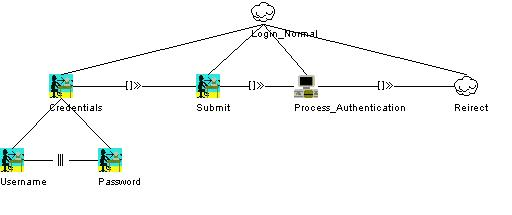
\includegraphics[width=0.9\textwidth]{/CTTxml/LoginNormal.jpg}
  \caption[Username / password login CTT]{CTT for logging in using a username and password}
\end{figure}

%-----------------------------------------------------------------------------------------------

\subsection{\label{subsec:loginFinger}Task scenario: login using a fingerprint}

Type: typical \\
Situation: the user whishes to login using his/her username and password. \\
Script:
\begin{enumerate}
\item System displays the four possible login methods.
\item User pushes the button to login using a fingerprint.
\item System displays a circle to indicate where the user has to put his finger.
\item User pushes his finger on the given spot.
\item System validates the fingerprint.
\begin{itemize}
\item \textbf{Wrong:} system shows a feedback message that the user is not authorized to the system, thus not authorized to make an appointment.
\item \textbf{Correct:} system redirects the user to the  confirmation screen.
\end{itemize}
\end{enumerate}

\begin{figure}[H]
\centering
    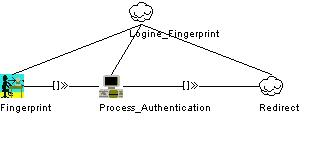
\includegraphics[width=0.9\textwidth]{/CTTxml/LoginFingerprint.jpg}
  \caption[Fingerprint login CTT]{CTT for logging in using a fingerprint}
\end{figure}

%---------------------------------------------------------------------------------------------------

\subsection{\label{subsec:loginNFC}Task scenario: login using QR code}

Type: typical \\
Situation: the user whishes to login by scanning a QR code \\
Script:
\begin{enumerate}
\item System displays the four possible login methods.
\item User pushes the button to login using a QR code.
\item System displays the generated QR code.
\item User scans the QR code using his smartphone.
\item (Authentication takes place in the smartphone.)
\begin{itemize}
\item \textbf{Wrong:} system receives the error that the user is not authenticated and thus, the system shows a feedback message that the user is not authorized to the system, thus not authorized to make an appointment.
\item \textbf{Correct:} system redirects the user to the ageinda.
\end{itemize}
\end{enumerate}

\begin{figure}[H]
\centering
    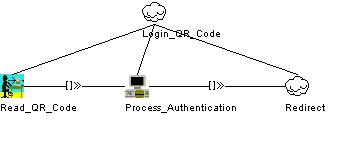
\includegraphics[width=0.9\textwidth]{/CTTxml/LoginQR.jpg}
  \caption[QR code login CTT]{CTT for logging in using QR code}
\end{figure}

%-------------------------------------------------------------------------------------------------

\subsection{\label{subsec:loginSpeech}Task scenario: login using speech}

Type: typical \\
Situation: the user whishes to login using voice authentication (speech). \\
Script:
\begin{enumerate}
\item System displays the four possible login methods.
\item User pushes the button to login using speech.
\item System outputs a spoken message states that the user can talk.
\item User provides his name in a spoken manner.
\item System validates the user's voice input.
\begin{itemize}
\item \textbf{Wrong:} system outputs an error sound.
\item \textbf{Correct:} system outputs an informational sound and redirects the user to the  confirmation screen.
\end{itemize}
\end{enumerate}

\begin{figure}[H]
\centering
    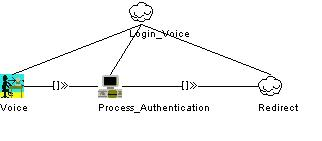
\includegraphics[width=0.9\textwidth]{/CTTxml/LoginVoice.jpg}
  \caption[Voice login CTT]{CTT for logging in using speech / voice}
\end{figure}

\begin{figure}[H]
\centering
    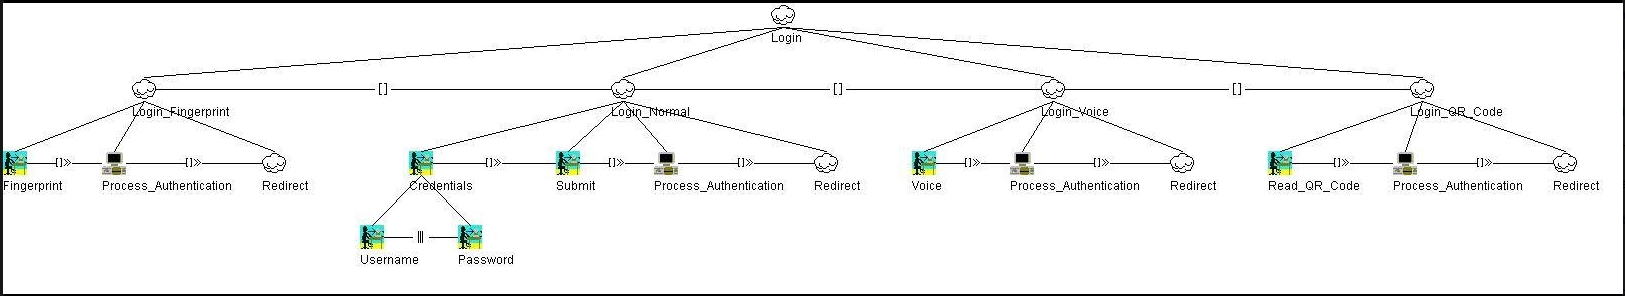
\includegraphics[width=1.4\textwidth, angle=90]{LoginComplete.png}
  \caption[Login CTT]{\label{fig:Login}Complete login CTT overview}
\end{figure}

%--------------------------------------------------------------------------------------

\subsection{Task scenario: logout}

Type: exceptional \\
Situation: the user whishes to logout. \\
Script:
\begin{enumerate}
\item User presses the logout button.
\item System shows a confirmation screen.
\begin{itemize}
\item \textbf{Confirm:} system redirects user to the begin screen and the user will be logged out.
\item \textbf{Cancel:} system redirects the user to the agenda page of the primary user.
\end{itemize}
\end{enumerate}

\begin{figure}[H]
\centering
    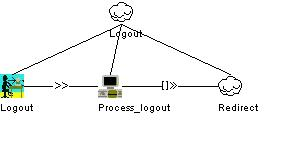
\includegraphics[width=0.8\textwidth]{Logout.jpg}
  \caption[Logout CTT]{\label{fig:Logout}Logout CTT}
\end{figure}

%--------------------------------------------------------------------------------------------------------

\subsection{Task scenario: show agenda of primary user}

\label{subsec:agenda}Type: typical \\
Situation: the user whishes to view  the agenda and planning of the primary user. \\
Script:
\begin{enumerate}
\item User pushes the show agenda button.
\item System displays the four possible login methods.
\item User logs in as explained in task scenarios \ref{subsec:loginPass}, \ref{subsec:loginFinger}, \ref{subsec:loginSpeech} and \ref{subsec:loginNFC}.
\item System redirects user to the agenda and planning of the primary user.
\end{enumerate}

\begin{figure}[H]
\centering
    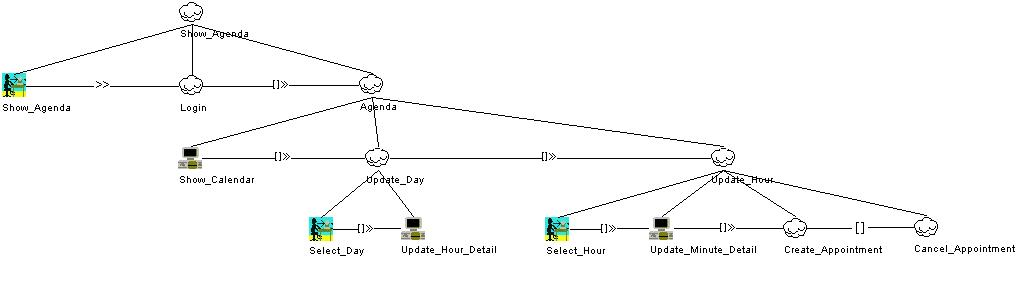
\includegraphics[width=1\textwidth]{ShowAgenda.jpg}
  \caption[Display agenda CTT]{\label{fig:ShowAgenda}CTT to display the user's agenda.}
\end{figure}

%----------------------------------------------------------------------------------------------------------

\subsection{Task scenario: select a day}

\label{subsec:day}Type: typical \\
Situation: the user whishes to select a cerain day  of the primary user's calendar. \\
Script:
\begin{enumerate}
\item User selects the month on the calendar using the buttons to scroll through the months.
\item System updates the calendar showing the selected month.
\item User selects the day by clicking on it.
\item System updates the rightside pane with the detailed information of that day.
\end{enumerate}

%--------------------------------------------------------------------------------------------------------

\subsection{Task scenario: select the time}

\label{subsec:hour}Type: typical \\
Situation: the user whishes to select a cerain hour  of the primary user's calendar at a certain day. \\
Script:
\begin{enumerate}
\item User selects the day on the calendar as explained in task scenario \ref{subsec:day}.
\item User selects the hour using the up and down arrows.
\item System updates the minute list.
\item User can now scroll through that hour.
\end{enumerate}

\begin{figure}[H]
\centering
    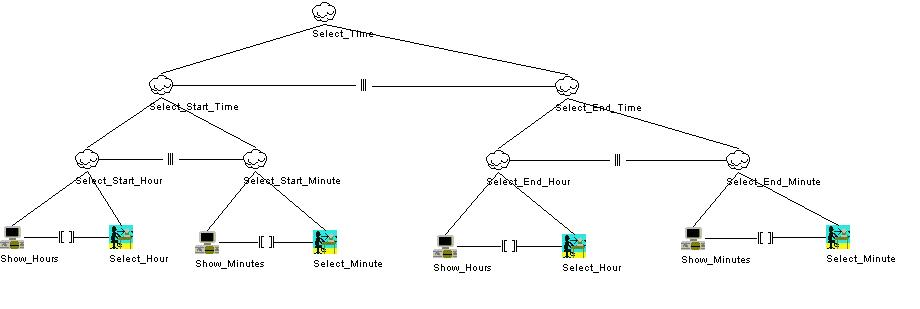
\includegraphics[width=0.9\textwidth]{/CTTxml/SelectTime.jpg}
  \caption[Select time CTT]{\label{fig:SelectTimeCTT}CTT for selecting the desired time}
\end{figure}

%------------------------------------------------------------------------------------------------

\subsection{Task scenario: conflicting appointment}


\label{subsec:conflict}Type: typical \\
Situation: a conflict was detected while making an appointment. \\
Script:
\begin{enumerate}
\item System will collor the make appointment screen in red.
\item User will have to choose another time for the appointment.
\item System restores the original colors of the window if no conflict is detected.
\end{enumerate}

\begin{figure}[H]
\centering
    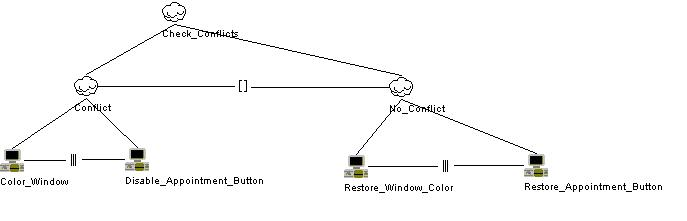
\includegraphics[width=0.9\textwidth]{/CTTxml/Conflict.jpg}
  \caption[Conflict appointment CTT]{\label{fig:ConflictAppointment}CTT for conflicting appointments}
\end{figure}

%---------------------------------------------------------------------------------------------

\subsection{Task scenario: make an appointment}


\label{subsec:appointment}Type: typical \\
Situation: the user whishes to make an appointment. \\
Script:
\begin{enumerate}
\item User presses the show agenda button.
\item User selects the month and day of when he wants an appointment as in task scenario \ref{subsec:day}.
\item User can now choose the exact starting hour of the appointment as in task scenario \ref{subsec:hour}.
\item System will redirect user to another page showing the starting hour and end hour in scrollable lists.
\item User chooses the end time and can change the start time if he/she wishes to.
\item System checks for conflicts and will take the appropriate actions.
\item User clicks on the button to make an appointment.
\item System redirects user to the confirmation screen.
\end{enumerate}

\begin{figure}[H]
\centering
    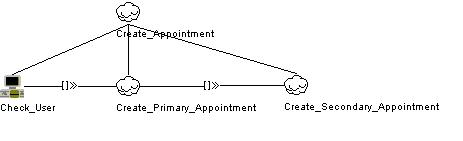
\includegraphics[width=0.9\textwidth]{CreateAppointment.jpg}
  \caption[Create appointment CTT]{\label{fig:CreateAppointment}CTT to create an appointment}
\end{figure}

\subsection{Task scenario: confirmation screen}

Type: typical \\
Situation: the user whishes to make an appointment. \\
Script:
\begin{enumerate}
\item User makes an appointments as in task scenario \ref{subsec:appointment}.
\item System shows the confirmation message.
\item User can now choose to confirm the appointment or can cancel it.
\item System will redirect the user
\begin{itemize}
\item \textbf{Confirm:} system shows a confirmation message and system redirects user to the begin screen and the user will be logged out automatically.
\item \textbf{Cancel:} system redirects the user to the agenda page of the primary user.
\end{itemize}
\end{enumerate}


\subsection{Task scenario: cancel an appointment}

Type: typical \\
Situation: the user whishes to cancel an appointment. \\
Script:
\begin{enumerate}
\item User presses the show agenda button as in task scenario \ref{subsec:agenda}.
\item User selects the month and day of when he wants an appointment as in task scenario \ref{subsec:day}.
\item User can now choose the exact starting hour of the appointment as in task scenario \ref{subsec:hour}.
\item User chooses his own appointment, which is colored in another color.
\item System will redirect the user to a deletion confirmation page.
\item User clicks on delete to actually delete the appointment.
\item System redirects user
\begin{itemize}
\item \textbf{Confirm:} system shows a confirmation message and system redirects user to the begin screen and the user will be logged out automatically.
\item \textbf{Cancel:} system redirects the user to the agenda page of the primary user.
\end{itemize}
\end{enumerate}

\begin{figure}[H]
\centering
    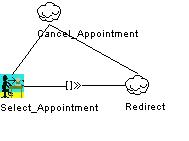
\includegraphics[width=0.6\textwidth]{CancelAppointment.jpg}
  \caption[Cancel appointment CTT]{\label{fig:CancelAppointment}CTT to cancel an appointment}
\end{figure}


\section{Task scenario: primary users}
A primary user has all the same functionalities as the secondary users. They have a few more privileges that we will explain in this section.


\subsection{Task scenario: conflicting appointment}


\label{subsec:conflictPrimary}Type: typical \\
Situation: a conflict was detected while making an appointment. \\
Script:
\begin{enumerate}
\item System will check where the conflict happened. Either it happend in the room section or it happened in the select primary users section.
\item System will color the conflicted section red.
\item User will have to resolve the conflict be either choosing a new room or change some people from the meeting.
\item System restores the original colors of the window if no conflict is detected.
\end{enumerate}


\subsection{Task scenario: create appointment on his/her own screen}


Type: typical \\
Situation: the user whishes to create an appointment. \\
Script:
\begin{enumerate}
\item User presses the show agenda button as in task scenario \ref{subsec:agenda}.
\item User selects the month and day of when he wants an appointment as in task scenario \ref{subsec:day}.
\item User can now choose the exact starting hour of the appointment as in task scenario \ref{subsec:hour}.
\item System will redirect user to another page showing the starting hour and end hour in scrollable lists.
\item User chooses the end time and can change the start time if he/she wishes to.
\item User can add other primary users to the appointment and select a room for the meeting.
\item System checks for conflicts and will take the appropriate actions as explained in \ref{subsec:conflictPrimary}
\item User clicks on the button to make an appointment.
\item System redirects user to the confirmation screen.
\end{enumerate}



\subsection{Task scenario: create a break}


Type: typical \\
Situation: the user whishes to take a break. \\
Script:
\begin{enumerate}
\item User presses the show agenda button as in task scenario \ref{subsec:agenda}.
\item User selects the month and day of when he wants an appointment as in task scenario \ref{subsec:day}.
\item User can now choose the exact starting hour of the appointment as in task scenario \ref{subsec:hour}.
\item System will redirect user to another page showing the starting hour and end hour in scrollable lists.
\item User has to select the break tab of the window.
\item System will display the content of the new tab.
\item User chooses the type of break and the time he/she is going to take a break.
\item User clicks on the button to create a break.
\item System redirects user to the begin page and automatically logs the user out. \\ \\
\end{enumerate}

\begin{figure}[H]
\centering
    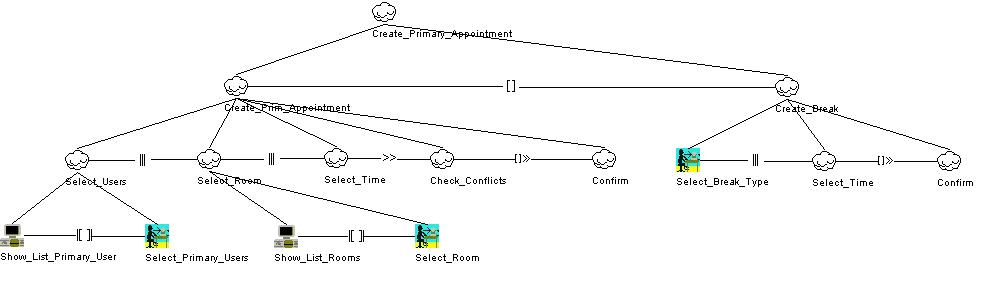
\includegraphics[width=1\textwidth]{CreatePrimaryAppointment.jpg}
  \caption[Primary user makes his own appointment]{\label{fig:PrimaryUserAppointment}CTT of the primary user making an appointment on his own screen. I.e., he arranges a meeting. Or making a break.}
\end{figure}

\newpage

\section{Task scenario: big WISE screen}


\subsection{Task scenario: searching for the primary users}


\label{subsec:alphabetic}Type: typical \\
Situation: the user whishes to find a primary user by name. \\
Script:
\begin{enumerate}
\item User inserts part of the name or the whole name in the search field.
\item User presses the search button.
\item System updates the screen and displays the name, availability and room of the searched 
person.
\end{enumerate}

\begin{figure}[H]
\centering
    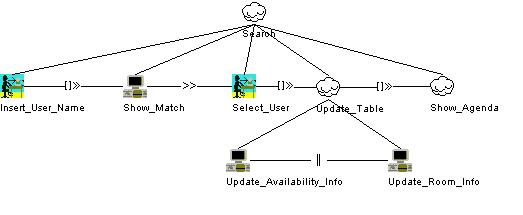
\includegraphics[width=1\textwidth]{Search_User.jpg}
  \caption[Search a user CTT]{\label{fig:SearchUser}CTT to search for a user}
\end{figure}


\subsection{Task scenario: creating an appointment using the big WISE screen}


Type: typical \\
Situation: the user whishes to create an appointment using the big WISE screen. \\
Script:
\begin{enumerate}
\item User selects the primary user he's interested in.
\item System updates the screen and will ask the user to log in.
\item User can now see the aganda and calendar of the selected user and can create an appointment as explained in \ref{subsec:appointment}
\end{enumerate}

\begin{figure}[H]
\centering
    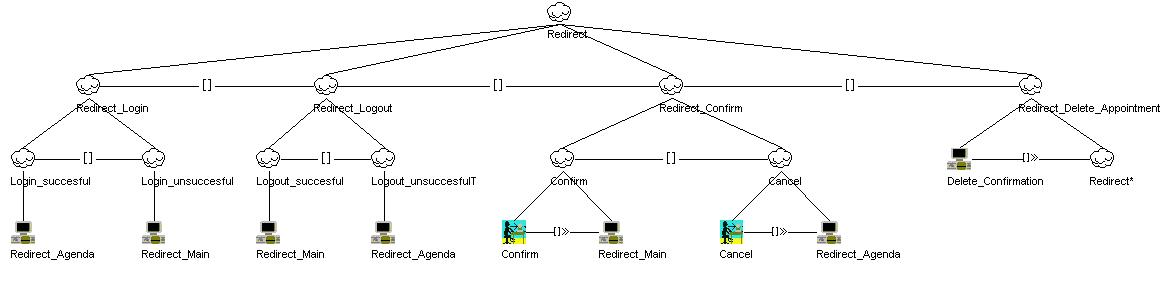
\includegraphics[width=1\textwidth]{Redirect.jpg}
  \caption[Redirect CTT]{\label{fig:CreateAppointment}CTT to redirect the user to the begin screen}
\end{figure}


\section{User Object Models}

\subsection{General information}

As explained in the user definition, we have two kinds of users: primary users and secondary users. The primary users are all the WISE members from the WISE lab. The secondary users are the rest of the VUB, that is, everyone with a netID. They can be students or even someone from another lab or faculty.

Secondary users can only make appointments with the professor/assistant of whom the screen belongs to. Primary users on the other hand can create appointments and can choose who they will meet (one person or a group of persons) and in what room the meeting will take place. In other words, primary users can plan meetings. 
Therefore, we designed the model in a way that one can find the attendees of the appointment. The attendees for the primary users can be a list of persons or a single person. For the secondary users the attendees can only be the primary user they want to meet.

Primary users can also add special breaks on the calendar so someone who passes by his office can see why he is unavailable. It can be added only by the primary user. Like an appointment, these breaks have a beginning and end time. \\ \\
The User Object Model is provided in figure \ref{fig:UserObjectModel}.

\subsection{Models}

\begin{figure}[H]
\centering
    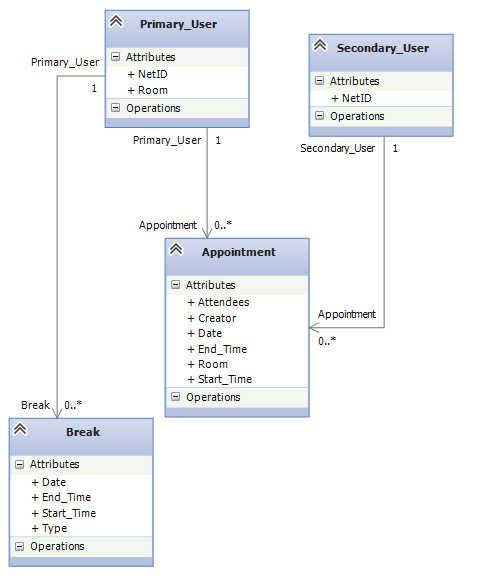
\includegraphics[width=1\textwidth]{UserObjectModels.png}
  \caption[User Object Model]{\label{fig:UserObjectModel}User Object Model}
\end{figure}

\chapter{Style guide}

\section{Standards for window interaction}

\subsection{Opening}

First, notice that there is no distinction between the big WISE screen and the little screen hanging next to the door of the professor or assistant. When a window will open on both of the displays, it will pop up right on the spot / place where it is meant to be. 

\subsection{Closing}

When a window is not needed anymore, it will just close the same way as it has been opened: by disappearing immediately (the opposite of popping up).

\section{Standard window layout}

The first screen contains a button to display the calendar of the primary user. Once clicked on it, one will be redirected to a pop up screen that gives the possibility to log in. There exists four possibilities to login: the user can login using a username/password combination, using voice, fingerprint and/or QR-code. Once logged in, the user is automatically redirected to the agenda page. \\ \\
Note that before logging in, one can already see a button in the upper right corner. This is the close button and is used to go back to the main page. Figure \ref{fig:CloseButton} gives a general impression of what the button looks like.
\begin{figure}[H]
\centering
    
\includegraphics[width=0.2\textwidth]{CloseButton.png}
  \caption[Close Button]{\label{fig:CloseButton} Close button}
\end{figure}

Once logged in, the user will be redirected to the calendar page of the primary user, that is, the calendar page of the professor or assistant. This is where a log out button is available. This button will sign off the user and redirect him to the main screen. Figure \ref{fig:SignOutButton} gives a general impression of what the button looks like.
\begin{figure}[H]
\centering
    
\includegraphics[width=0.2\textwidth]{SignOff.png}
  \caption[Sign out Button]{\label{fig:SignOutButton} Sign out button}
\end{figure}

In the bottom left corner a button will be available to return to the previous page. Figure \ref{fig:GoBackButton} gives a general impression of what the button looks like.
\begin{figure}[H]
\centering
    
\includegraphics[width=0.2\textwidth]{Back.png}
  \caption[Go Back Button]{\label{fig:GoBackButton} Go back button}
\end{figure}

The the first screen is the main page. Here one can see if the professor / assistant (the primary user) is present or not.  There is also a possibilitie to view the calendar of the primary user by tapping on the button ``make an appointment''. Figure \ref{fig:BeginScreen} gives a general impression of what the button looks like.
\begin{figure}[H]
\centering
    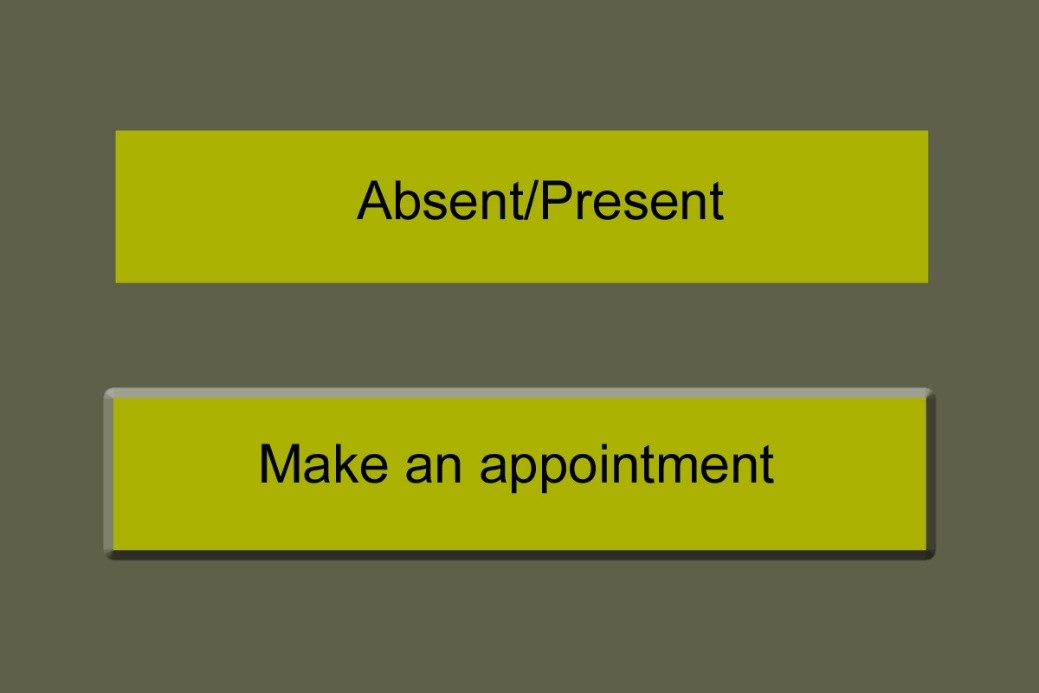
\includegraphics[width=0.8\textwidth]{Main.jpg}
  \caption{\label{fig:BeginScreen} The begin / main screen}
\end{figure}

Tapping the button will make a pop up screen appear with four possible ways to log in. A blur effect is also used to `blur out' the underlying screen. Figure \ref{fig:LoginScreen} gives a general impression of what the button looks like.
\begin{figure}[H]
\centering
    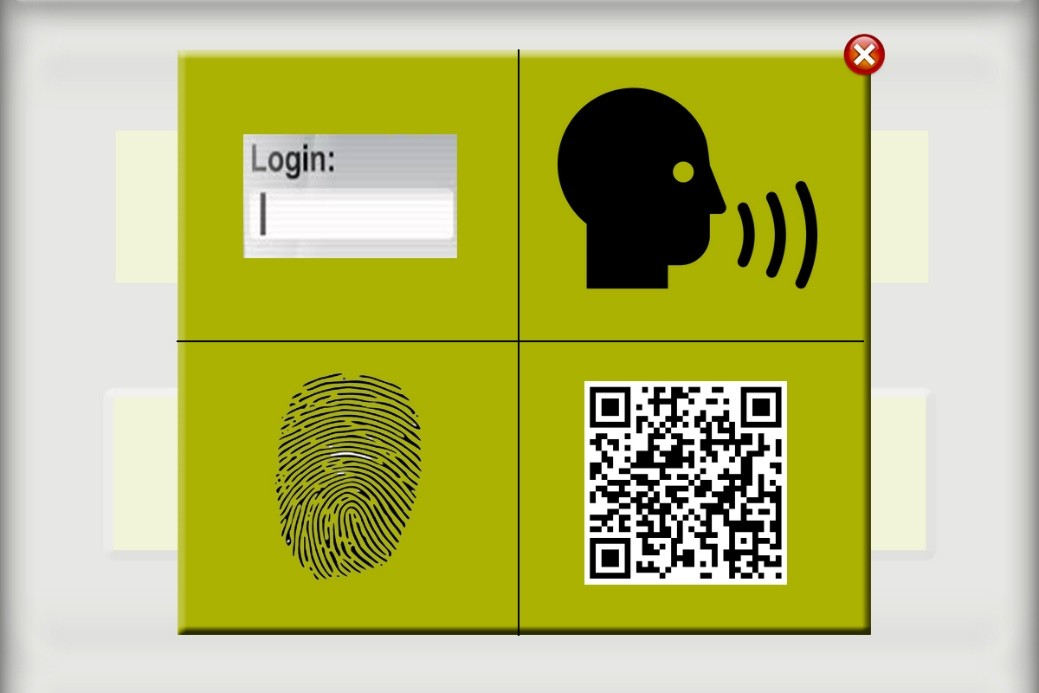
\includegraphics[width=0.8\textwidth]{Login.jpg}
  \caption[Login screen]{\label{fig:LoginScreen} The login screen showing the four possible login methods. Note the blur effect.}
\end{figure}

When a user chooses to login using a name / password combination, he gets to see another pop up screen with two text fields to fill in a netID and a password, because of the text input, there will also be a keyboard available to type. If the user wants to choose another way to log in, he can always do so by selecting the return button that will lead him to the four different options to log in.

\begin{figure}[H]
\centering
    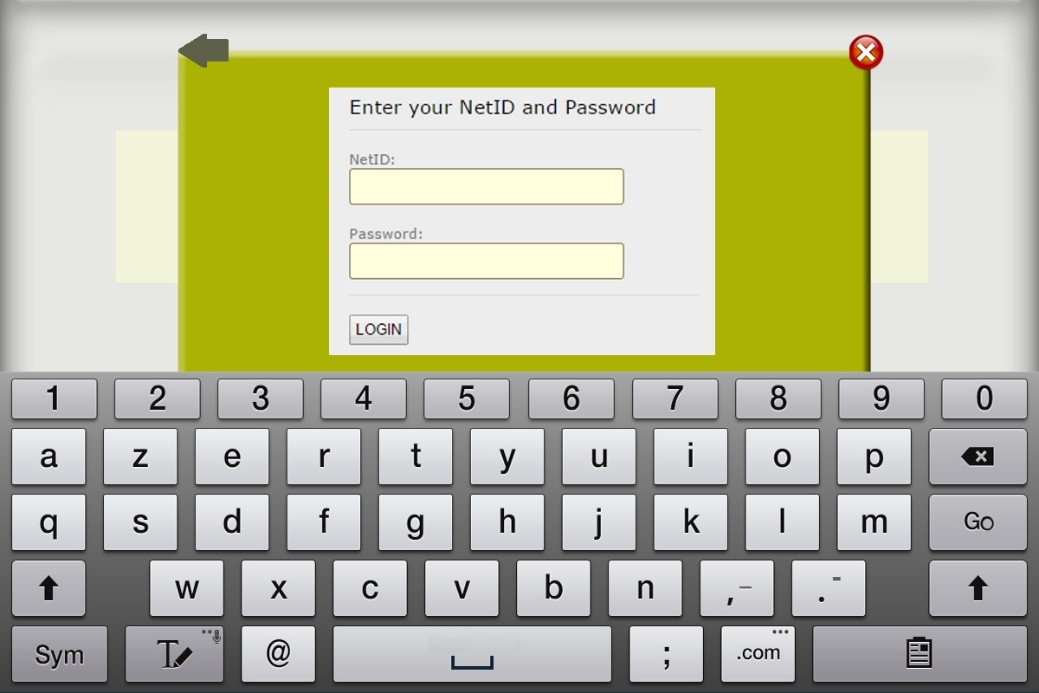
\includegraphics[width=0.7\textwidth]{Textfield.jpg}
  \caption[Name / password combination login]{\label{fig:LoginScreen2}The screen where a user can login using his VUB netID and password. Note the blur effect and the virtual keyboard.}
\end{figure}

When the user, for example, deletes an appointment, a confirmation screen will be shown. The purpose of this screen is to warn the user for the upcoming action. Therefore, a confirmation screen consists of two components: the confirmation message itself, two buttons and an exclamation mark symbol. The meaning of the confirmation message is straightforward; the two buttons are a ``yes'' and ``no'' button, to actually confirm and proceed with the action and to return to the main page, respectively. 

\begin{figure}[H]
\centering
    
\includegraphics[width=0.2\textwidth]{Warning.png}
  \caption[Warning sign]{\label{fig:WarningSign} The warning sign}
\end{figure}

\begin{figure}[H]
\centering
    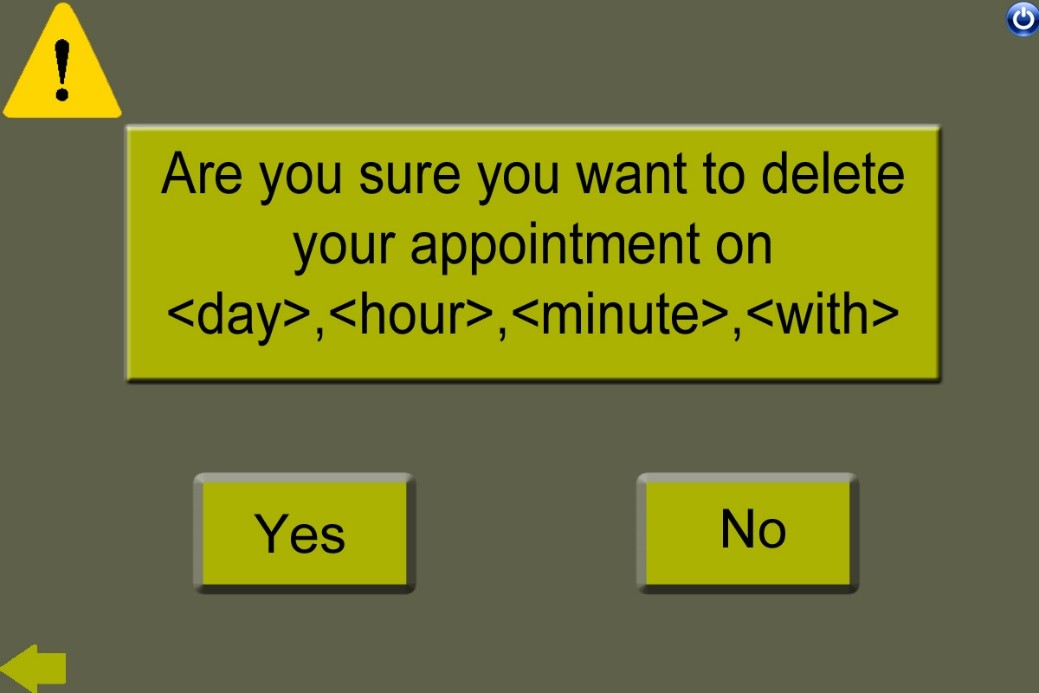
\includegraphics[width=0.8\textwidth]{Confirmation.jpg}
  \caption[Confirmation screen]{\label{fig:ConfirmationScreen} The confirmation screen}
\end{figure}

For blind people or visually impaired people there exists an application called TalkBack which is part of the Google Android Accessibility Service. This application is built so they can hear what they have to do. To enable this one needs to do the following:

\begin{figure}[H]
\centering
    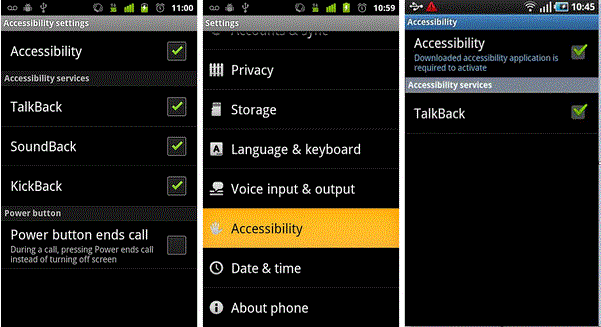
\includegraphics[width=0.8\textwidth]{Talkback.png}
  \caption[Talkback]{\label{fig:Talkback} Talkback.}
\end{figure}

Of course, if a user is logged in any other way than the speak recognition manner, the TalkBack application will automatically be disabled.
Once logged in, the user will be redirected to the calendar page. The header contains a label where the user can see in which section he is. On the upper right corner of the page one can log out by clicking the log out button right above the current time.

\section{Standards for menus and push buttons}

As previously mentionend, every time a pop up window appears, the screen a user was on will be blurry.
We also will use the hover effect. For example, when a user hovers his cursor over the sign off button, the function of the button will appear.
Navigation buttons will always appear in the left bottom corner in the footer. The close/sign off button will be placed in the right upper corner.

The WISE screen contains a search box with autocomplete function where one can look up a member. His or her availability will be shown below with the information needed. If that person is available, one can see where the specified user is at the moment. On the other hand, if he is not available a reason is shown why he is not. One example could be because the person is on a coffee break.

\begin{figure}[H]
\centering
    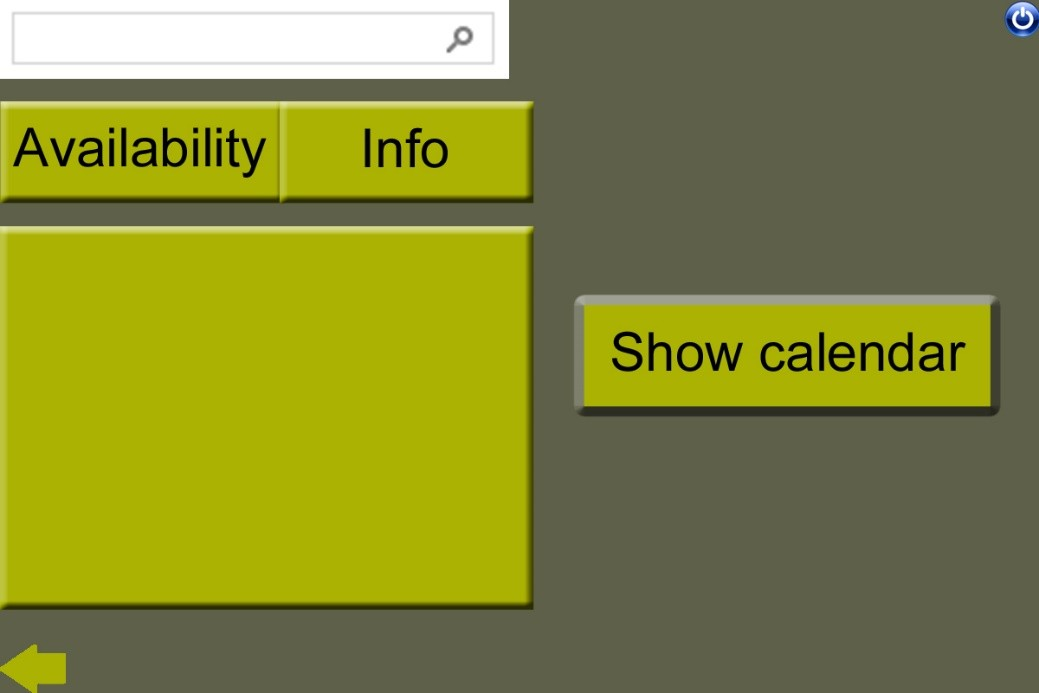
\includegraphics[width=0.8\textwidth]{Wise.jpg}
  \caption[WISE screen]{The big WISE screen}
\end{figure}

\section{Standards for menus and gestures for touch screen devices}

Large buttons will be used to make it easier to use on touch screen devices. Only icons will be used instead of icons with a label for the convenience.
For example, for the sign off button, we make use of an icon and not of a button with text: 

\begin{figure}[H]
\centering
    
\includegraphics[width=0.2\textwidth]{SignOff.png}
  \caption[Log off button]{The log out button}
\end{figure}

\section{Standards for use of keyboard keys}

When a user fills in a textbox there exists a button ``go'' that will function like the tab key on a regular keyboard.

\begin{figure}[H]
\centering
    
\includegraphics[width=0.2\textwidth]{GO.png}
  \caption[Go button]{The go button}
\end{figure}

\newpage

For example: when a person wants to log in using his username / password combination. Instead of tapping the next textbox, he clicks on the button ``next'' that will automatically move his cursor to the next textbox, is this case the password. When the user clicks (touches) ``next'' after filling in his password, the cursor moves to the button ``login'' and gets the function ``enter''. This is another way to select an item when the keyboard is available. Figure \ref{fig:function} illustrates this.

\begin{figure}[H]
\centering
    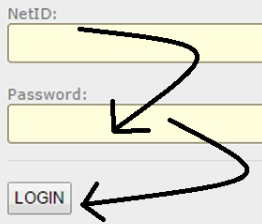
\includegraphics[width=0.5\textwidth]{GO2.png}
  \caption[Function go button]{\label{fig:function}Function go button}
\end{figure}

\section{Standards for use of window controls, and mapping of data types to window controls}

To represent date and time, a calendar will be used to select the date and a spinner to select the desired time. In the spinner, the availability status will automatically be shown next to the time. The item that resides in the middle of the spinner, is the item currently selected. The other items will be shown in grey. The middle item is colored in black. 

\begin{figure}[H]
\centering
    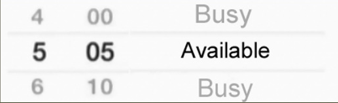
\includegraphics[width=0.3\textwidth]{Spinner.png}
  \caption[The spinner]{The spinner}
\end{figure}

When the secondary user wants to make an appointment, he gets to see the calendar below:

\begin{figure}[H]
\centering
    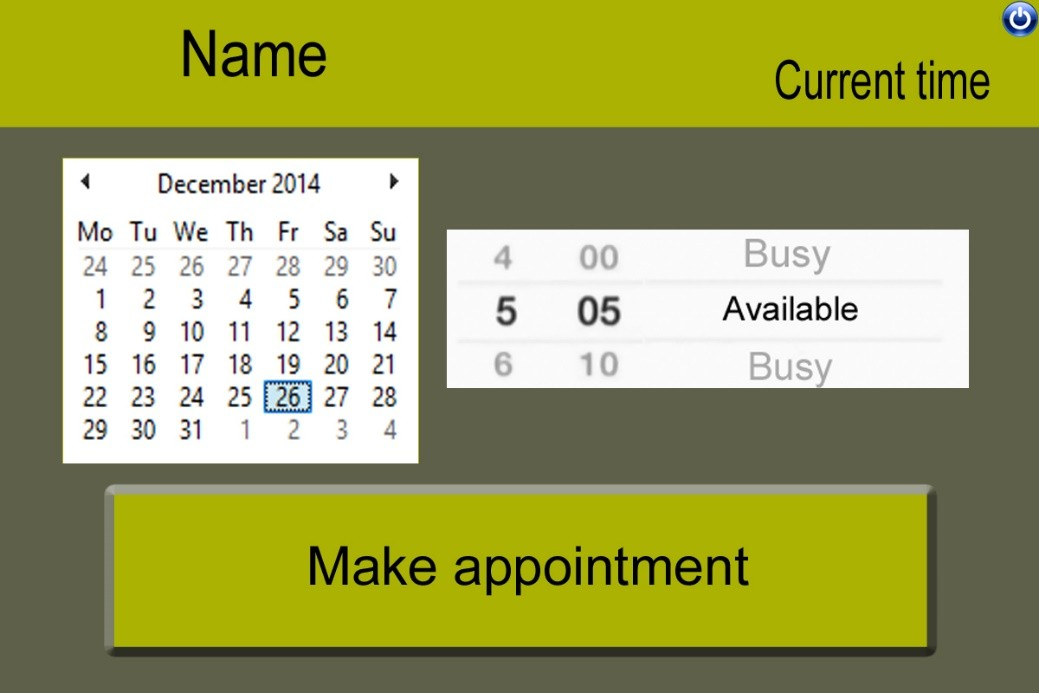
\includegraphics[width=0.7\textwidth]{Calendar.jpg}
  \caption[The calendar]{The calendar}
\end{figure}

For the primary user, following screens exist: when he wants to make an appointment with multiple members, he can do so by selecting multiple members in the left column and add them in the right column.

\begin{figure}[H]
\centering
    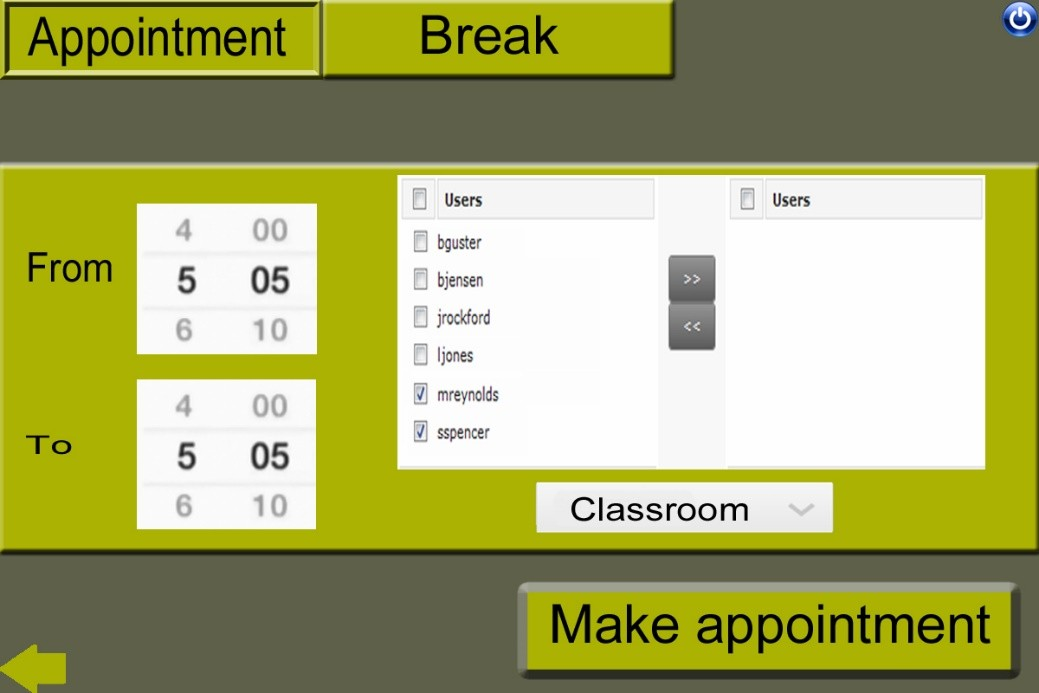
\includegraphics[width=0.7\textwidth]{Appointment.jpg}
  \caption[Appointment primary user]{The primary user can arrange meetings with peer professors / assistants.}
\end{figure}

\newpage

A break tab exist for primary users. This tab gives users the opportunity to plan breaks. There exist four possibilities: a lunch break, toilet break, coffee break and smoking break.

\begin{figure}[H]
\centering
    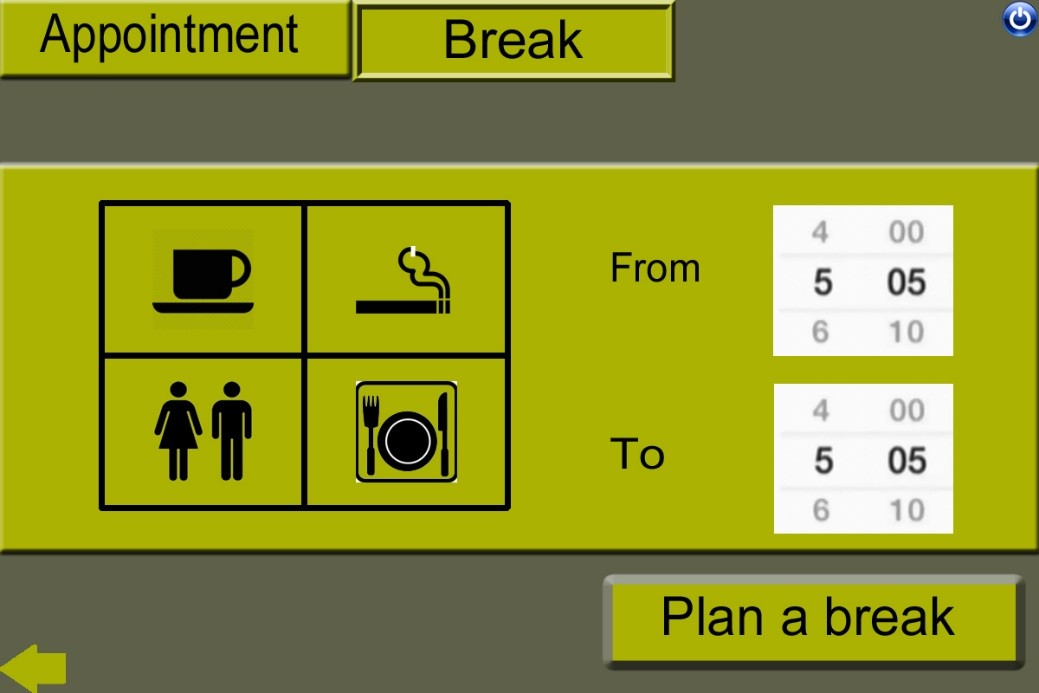
\includegraphics[width=0.7\textwidth]{Break.jpg}
  \caption[Take a break]{Planning a break}
\end{figure}

When the primary user taps a button (appointment or break), you will see that the button is pressed. The body will change depending on which button is tapped. Below an example of a button pressed

\begin{figure}[H]
\centering
    
\includegraphics[width=0.3\textwidth]{AppointmentButton.png}
  \caption[Button pressed]{Pressed button}
\end{figure}

Below there is an example of a button that is not pressed on: 

\begin{figure}[H]
\centering
    
\includegraphics[width=0.3\textwidth]{BreakButton.png}
  \caption[Normal button]{Normal, usual button}
\end{figure}

\newpage

\section{Standard use of color, type and fonts}

For the main screen, the background colour is \#ABB202 with the colour of the labels being \#5F604A. These are based on the VUB colours for consistency reasons. The font is sans-serif: Arial.

For the headers in the wizard the sans-serif style Arial with 30pt is used.
Colours will be used to give some information to the user as well. In the main page of the application, the status of the primary user will be colored in red if he is unavailable or in green if he is available. If the user is unavailable, an icon will appear so it is clear at a glance that the user is on a coffee break, in a meeting,\ldots. \\ \\
All the text, that is, the text on the buttons, the text on the calendar, \ldots are in the color \#000000. The background color of the warning sign is in the color \#AB9F00.

The colors of the the log out button are the following: \#01247B and \#799EF9, with \#FFFFFF being used for the actual sign. For the closing button, following colors are used: \#990000 for the background and \#FFFFFF for the white cross.

\section{Standards for common user objects}

There exist four possibilities. The first option is to log in with a netID and a password. As soon as a text field is selected, a keyboard will appear on the screen.

\begin{figure}[H]
\centering
    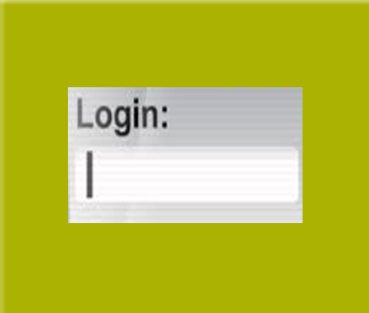
\includegraphics[width=0.3\textwidth]{NamePass.png}
  \caption[Name / password login]{Login using name / password combination}
\end{figure}

The second option is for visually impaired or blind people: speak recognition.

\begin{figure}[H]
\centering
    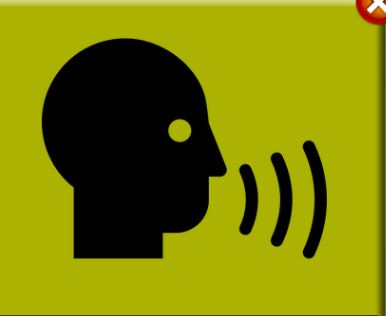
\includegraphics[width=0.3\textwidth]{Speak.png}
  \caption[Speach icon]{The speach icon}
\end{figure}

Next option is the ability to use fingerprint scanning.

\begin{figure}[H]
\centering
    
\includegraphics[width=0.3\textwidth]{Fingerprint.png}
  \caption[Fingerprint icon]{The fingerprint icon}
\end{figure}

Finally, there exists an option to use QR code because of the new concept BYOD (= Bring Your Own Device). Most people will have their own smartphone or other mobile device and we want to give them the opportunity to use this. This way, users can scan this code with their mobile devices and if so, they will be redirected to the page where they can make his or her appointment.

\begin{figure}[H]
\centering
    
\includegraphics[width=0.3\textwidth]{Qr.png}
  \caption[QR icon]{The QR icon}
\end{figure}

Icons are being used to represent the different types of breaks for the primary user. These breaks include: coffee break, smoking break, toilet break and lunch break. The user has to tap the icon to make his choice. The icon will light up when selected. 

\begin{figure}[H]
\centering
    
\includegraphics[width=0.3\textwidth]{CoffeeBreak.png}
  \caption[Coffee icon]{The coffee break icon}
\end{figure}

\begin{figure}[H]
\centering
    
\includegraphics[width=0.3\textwidth]{SmokingBreak.png}
  \caption[The spinner]{The smoking break icon}
\end{figure}

\begin{figure}[H]
\centering
    
\includegraphics[width=0.3\textwidth]{ToiletBreak.png}
  \caption[The spinner]{The toilet break icon}
\end{figure}

\begin{figure}[H]
\centering
    
\includegraphics[width=0.3\textwidth]{LunchBreak.png}
  \caption[The spinner]{The lunch break icon}
\end{figure}

This concludes the style guide.

%--------------------------------------------------------------------------
% DESIGN
%--------------------------------------------------------------------------

\chapter{Design}

We will apply the task-driven design technique on each of the CTT's. The MARIAE tool has been used to create the enable task sets of each of the CTT's. For informational purposes, the task description with the CTT will be given as well. On top of that, some design mockups are also supplied. Note however that these are just mockups, not the final (prototype) design. We provided them just to give the reader a general impression of how the final design could look like.

\section{\label{subsec:loginPass}Login using username and password}

As previously mentioned, four ways to login exist. The user can choose between logging in using his VUB netID in combination with his VUB password, or he can opt to use his fingerprint to login. But it is also possible to login by speaking to the device or using a QR code. We will describe them all four seperately using CTT's. Thus, for each login method, a CTT is provided in combination with the task sets.

\subsection{Task description and CTT}

When a user wants to login using his VUB netID and VUB password, he chooses the appropriate login method listed by the system, after which a new window pops up with two textfields. One to enter the username and one to enter the password. When the user taps on one textfield, a virtual keyboard is shown to input the desired text. After the username en password have been provided, the system validates the credentials and the user receives either an error message, or in case everything went well, he is redirected to the agenda.

Type: typical \\
Situation: the user whishes to login using his/her username and password. \\
Script:
\begin{enumerate}
\item System displays the four possible login methods.
\item User pushes the button to login using a username and password.
\item System shows two textfields and a virtual keyboard.
\item User provides his username and password.
\item System validates the login.
\begin{itemize}
\item \textbf{Wrong:} system shows a feedback message that the user is not authorized to the system, thus not authorized to make an appointment.
\item \textbf{Correct:} system redirects the user to the agenda.
\end{itemize}
\end{enumerate}

\begin{figure}[H]
\centering
    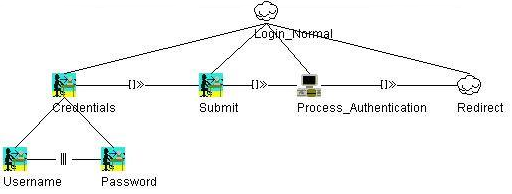
\includegraphics[width=0.8\textwidth]{LoginUsernamePass.png}
  \caption[Username / password CTT]{\label{fig:Logout}Login using name / password combination CTT}
\end{figure}

\subsection{Enabled task set}

\{Username,Password\},\{Submit,Process\_Authentication,Reirect\}

\subsection{First impression of the design}

\begin{figure}[H]
\centering
    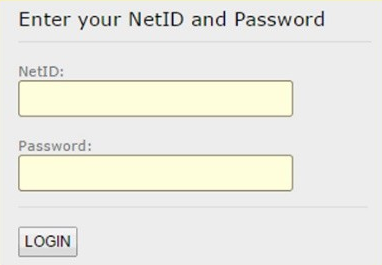
\includegraphics[width=0.5\textwidth]{LoginNoKeyboard.jpg}
  \caption[Login screen]{\label{fig:Login}Login using name / password combination}
\end{figure}

%-------------------------------------------------------------------------------------------

\newpage

\section{\label{subsec:loginFinger}Login using a fingerprint}

When a user wants to login using his fingerprint, he chooses the appropriate login method listed by the system, after which a new window pops up with a circle. After his fingerprint is taken, the system validates the credentials and the user receives either an error message, or in case everything went well, he is redirected to the agenda. This is described formally below:

\subsection{Task description and CTT}

Type: typical \\
Situation: the user whishes to login using his fingerprint. \\
Script:
\begin{enumerate}
\item System displays the four possible login methods.
\item User pushes the button to login using a fingerprint.
\item System displays a circle to indicate where the user has to put his finger.
\item User pushes his finger on the given spot.
\item System validates the fingerprint.
\begin{itemize}
\item \textbf{Wrong:} system shows a feedback message that the user is not authorized to the system, thus not authorized to make an appointment.
\item \textbf{Correct:} system redirects the user to the agenda.
\end{itemize}
\end{enumerate}

\begin{figure}[H]
\centering
    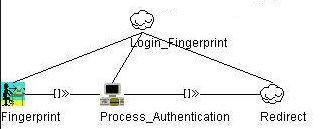
\includegraphics[width=0.8\textwidth]{LoginFingerprint.png}
  \caption[Fingerprint CTT]{\label{fig:Logout}Login using fingerprint CTT}
\end{figure}

\subsection{Enabled task set}

\{Fingerprint,Process\_Authentication,Redirect\}

%-----------------------------------------------------------------------------------

\newpage

\section{\label{subsec:loginNFC}Login using QR code}

\subsection{Task description and CTT}

When a user wants to login by means of a QR code, he chooses the appropriate login method listed by the system, after which a new window pops up with a QR code. The user scans this code with his smartphone, after which authentication takes place on the smartphone and the user receives either an error message, or in case everything went well, he is redirected to the agenda. This is described formally below:

Type: typical \\
Situation: the user whishes to login by scanning a QR code \\
Script:
\begin{enumerate}
\item System displays the four possible login methods.
\item User pushes the button to login using a QR code.
\item System displays the generated QR code.
\item User scans the QR code using his smartphone.
\item (Authentication takes place in the smartphone.)
\begin{itemize}
\item \textbf{Wrong:} system receives the error that the user is not authenticated and thus, the system shows a feedback message that the user is not authorized to the system, thus not authorized to make an appointment.
\item \textbf{Correct:} system redirects the user to the agenda.
\end{itemize}
\end{enumerate}

\begin{figure}[H]
\centering
    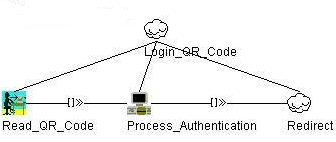
\includegraphics[width=0.8\textwidth]{LoginQR.png}
  \caption[QR CTT]{\label{fig:Logout}Login using QR code CTT}
\end{figure}

\subsection{Enabled task set}

\{Read\_QR\_Code,Process\_Authentication,Redirect\}

%-----------------------------------------------------------------------------

\newpage

\section{\label{subsec:loginSpeech}Login using speech}

\subsection{Task description and CTT}

If the user opts to login using voice / speech, he can do so by clicking the appropriate icon. Afterwards, the system outputs a spoken message indicating that the user is allowed to talk, that is, to authenticate himself using voice. When this is done, the system processes the voice, validates the user and in case of success, he is redirected to the agenda of the primary user.

Type: typical \\
Situation: the user whishes to login using voice authentication (speech). \\
Script:
\begin{enumerate}
\item System displays the four possible login methods.
\item User pushes the button to login using speech.
\item System outputs a spoken message states that the user can talk.
\item User provides his name in a spoken manner.
\item System validates the user's voice input.
\begin{itemize}
\item \textbf{Wrong:} system outputs an error sound.
\item \textbf{Correct:} system outputs an informational sound and redirects the user to the agenda.
\end{itemize}
\end{enumerate}

\begin{figure}[H]
\centering
    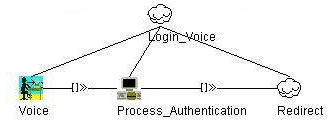
\includegraphics[width=0.8\textwidth]{LoginVoice.png}
  \caption[Speech CTT]{\label{fig:Logout}Login using speech CTT}
\end{figure}

\subsection{Enabled task set}

\{Voice,Process\_Authentication,Redirect\}

\subsection{First impression of the design}

\begin{figure}[H]
\centering
    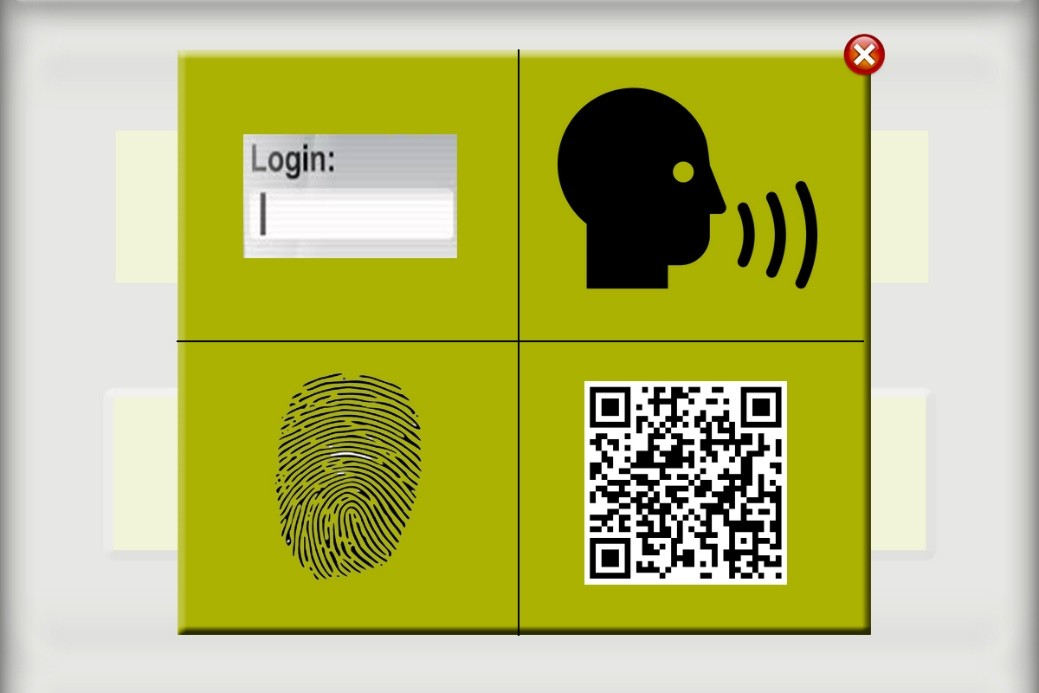
\includegraphics[width=0.8\textwidth]{Login.jpg}
  \caption[Login screen]{\label{fig:Login}Login with the four possibilities described above}
\end{figure}


%--------------------------------------------------------------------------------------------------------------

\newpage

\section{logging out}

\subsection{Task description and CTT}

Normally, a user will be logged out automatically when he makes an appointment, but of course a user can always choose to `force' this logout by pressing the logout button. This is why log out is being considered as exceptional.

If the user presses the logout button, the system shows a confirmation screen should the user tapped this button accidentally. There exist two actions of which the user can choose: either he confirms the logout, or he declines it. In the former case, the user is redirected to the main screen, wheras in the latter case, the logout windows just disappears and the user gets to see the last window he was on. This is written more formally below:\\ \\
Type: exceptional \\
Situation: the user whishes to logout. \\
Script:
\begin{enumerate}
\item User presses the logout button.
\item System shows a confirmation screen.
\begin{itemize}
\item \textbf{Confirm:} system redirects user to the begin screen and the user will be logged out.
\item \textbf{Cancel:} system redirects the user to the agenda page of the primary user.
\end{itemize}
\end{enumerate}

\begin{figure}[H]
\centering
    \includegraphics[width=0.7\textwidth]{Logout.jpg}
  \caption[Logout CTT]{\label{fig:Logout}Logout CTT}
\end{figure}

\subsection{Enabled task set}

\{Logout,Process\_Logout,Redirect\}

%-----------------------------------------------------------------------------------------------------------------------

\newpage

\section{Show the agenda of the primary user}

\subsection{Task description and CTT}

When the user wants to view the agenda of the primary user (that is, the professor / assistant) from within the main screen, he can do so by tapping the appropriate button, after which he is shown a request to authenticate himself. There, the user can choose from the four possible login methods as explained above. When authenticated successfully, the user is redirected to the actual agenda of the primary user. This process is described more formally below.

\label{subsec:agenda}Type: typical \\
Situation: the user whishes to view  the agenda and planning of the primary user. \\
Script:
\begin{enumerate}
\item User pushes the show agenda button.
\item System displays the four possible login methods.
\item User logs in as explained in task scenarios \ref{subsec:loginPass}, \ref{subsec:loginFinger}, \ref{subsec:loginSpeech} and \ref{subsec:loginNFC}.
\item System redirects user to the agenda and planning of the primary user.
\end{enumerate}

\begin{figure}[H]
\centering
    \includegraphics[width=1\textwidth]{ShowAgenda.jpg}
  \caption[Display agenda CTT]{\label{fig:ShowAgenda}CTT to display the user's agenda.}
\end{figure}

\subsection{Enabled task sets}

\{Press\_Show\_Agenda,Login,Show\_Calendar\},\{Select\_Day,Update\_Hour\_Detail\}, \\ \{Select\_Hour,Update\_Minute\_Detail,Create\_Appointment, Cancel\_Appointment\}


\subsection{First impression of the GUI}

\begin{figure}[H]
\centering
    \includegraphics[width=0.8\textwidth]{Calendar.jpg}
  \caption[The calendar]{\label{fig:ShowAgenda}The calendar.}
\end{figure}



%--------------------------------------------------------------------------------------------------------------

\newpage

\section{Conflicting appointment}

\subsection{Task description and CTT}

\label{subsec:conflict}Type: typical \\
Situation: a conflict was detected while making an appointment. \\
Script:
\begin{enumerate}
\item System will collor the make appointment screen in red.
\item User will have to choose another time for the appointment.
\item System restores the original colors of the window if no conflict is detected.
\end{enumerate}

\begin{figure}[H]
\centering
    \includegraphics[width=0.9\textwidth]{CheckConflicts.png}
  \caption[Check conflict CTT]{\label{fig:CheckConflict}CTT check and resolve a conflict}
\end{figure}

\subsection{Enabled task sets}

\{Color\_Window,Disable\_Appointment\_Button,Restore\_Window\_Color,Restore\_Appointment\_Button\}

%------------------------------------------------------------------------------------------------------------

\newpage

\section{Make an appointment}

\subsection{Task description and CTT}

\label{subsec:appointment}Type: typical \\
Situation: the user whishes to make an appointment. \\
Script:
\begin{enumerate}
\item User presses the show agenda button as in task scenario \ref{subsec:agenda}.
\item User selects the month and day of when he wants an appointment as in task scenario \ref{subsec:day}.
\item User can now choose the exact starting hour of the appointment as in task scenario \ref{subsec:hour}.
\item System will redirect user to another page showing the starting hour and end hour in scrollable lists.
\item User chooses the end time and can change the start time if he/she wishes to.
\item System checks for conflicts and will take the appropriate actions as explained in \ref{subsec:conflict}
\item User clicks on the button to make an appointment.
\item System redirects user to the confirmation screen.
\end{enumerate}

\begin{figure}[H]
\centering
    \includegraphics[width=0.9\textwidth]{CreateAppointment.jpg}
  \caption[Create appointment CTT]{\label{fig:CreateAppointment}CTT to create an appointment}
\end{figure}

\subsection{Enabled task sets}

\{Check\_User,Create\_Primary\_Appointment,Create\_Secondary\_Appointment\}

\subsection{First impression of the design}

\begin{figure}[H]
\centering
    \includegraphics[width=1\textwidth]{Appointment.jpg}
  \caption[Appointment screen]{\label{fig:Appointment}Screen to create an appointment.}
\end{figure}

%----------------------------------------------------------------------------------------------------------

\newpage

\section{Cancelling an appointment}

\subsection{Task description and CTT}

Type: typical \\
Situation: the user whishes to cancel an appointment. \\
Script:
\begin{enumerate}
\item User presses the show agenda button as in task scenario \ref{subsec:agenda}.
\item User selects the month and day of when he wants an appointment as in task scenario \ref{subsec:day}.
\item User can now choose the exact starting hour of the appointment as in task scenario \ref{subsec:hour}.
\item User chooses his own appointment, which is colored in another color.
\item System will redirect the user to a deletion confirmation page.
\item User clicks on delete to actually delete the appointment.
\item System redirects user
\begin{itemize}
\item \textbf{Confirm:} system shows a confirmation message and system redirects user to the begin screen and the user will be logged out automatically.
\item \textbf{Cancel:} system redirects the user to the agenda page of the primary user.
\end{itemize}
\end{enumerate}

\begin{figure}[H]
\centering
    \includegraphics[width=0.6\textwidth]{CancelAppointment.jpg}
  \caption[Cancel appointment CTT]{\label{fig:CancelAppointment}CTT to cancel an appointment}
\end{figure}

\subsection{Enabled task sets}

\{Select\_Appointment, Redirect\}

%------------------------------------------------------------------------------------------------

\newpage

\section{Conflicting appointment for the primary user}

\subsection{Task description and CTT}

\label{subsec:conflictPrimary}Type: typical \\
Situation: a conflict was detected while making an appointment. \\
Script:
\begin{enumerate}
\item System will check where the conflict happened. Either it happend in the room section or it happened in the select primary users section.
\item System will color the conflicted section red.
\item User will have to resolve the conflict be either choosing a new room or change some people from the meeting.
\item System restores the original colors of the window if no conflict is detected.
\end{enumerate}

\begin{figure}[H]
\centering
    \includegraphics[width=1\textwidth]{CTTxml/Conflict.jpg}
  \caption[Conflicting appointment]{\label{fig:ConflictingAppointment}CTT to resolve conflicts made during the process of making an appointment.}
\end{figure}

\subsection{Enabled task sets}

\{Color\_Window,Disable\_Appointment\_Button,Restore\_Window\_Color,Restore\_Appointment\_Button\}

%-------------------------------------------------------------------------------------------------

\newpage

\section{Primary user whishes to create an appointment on his own screen}

\subsection{Task description and CTT}

Type: typical \\
Situation: the user whishes to create an appointment. \\
Script:
\begin{enumerate}
\item User presses the show agenda button as in task scenario \ref{subsec:agenda}.
\item User selects the month and day of when he wants an appointment as in task scenario \ref{subsec:day}.
\item User can now choose the exact starting hour of the appointment as in task scenario \ref{subsec:hour}.
\item System will redirect user to another page showing the starting hour and end hour in scrollable lists.
\item User chooses the end time and can change the start time if he/she wishes to.
\item User can add other primary users to the appointment and select a room for the meeting.
\item System checks for conflicts and will take the appropriate actions as explained in \ref{subsec:conflictPrimary}
\item User clicks on the button to make an appointment.
\item System redirects user to the confirmation screen.
\end{enumerate}

\begin{figure}[H]
\centering
    \includegraphics[width=1\textwidth]{CreatePrimaryAppointment.jpg}
  \caption[Primary user makes his own appointment]{\label{fig:PrimaryUserAppointment}CTT of the primary user making an appointment on his own screen. I.e., he arranges a meeting.}
\end{figure}

\subsection{Enabled task sets}

\{Show\_List\_Primary\_User,Select\_Primary\_Users, \\ Show\_List\_Rooms,Select\_Room,Select\_Time,Check\_Conflicts,Select\_Break\_Type\}

%----------------------------------------------------------------------------------------

\newpage

\section{Task scenario: searching for the primary users on the big WISE screen}

\subsection{Task description and CTT}

\label{subsec:alphabetic}Type: typical \\
Situation: the user whishes to find a primary user by name. \\
Script:
\begin{enumerate}
\item User inserts part of the name or the whole name in the search field.
\item User presses the search button.
\item System updates the screen and displays the name, availability and room of the searched 
person.
\end{enumerate}

\begin{figure}[H]
\centering
    \includegraphics[width=1\textwidth]{Search_User.jpg}
  \caption[Search a user CTT]{\label{fig:SearchUser}CTT to search for a user}
\end{figure}

\subsection{Enabled task sets}

\{Insert\_User\_Name,Show\_Match\},\{Select\_User,Update\_Availability\_Info,Update\_Room\_Info,Show\_Agenda\}

%---------------------------------------------------------------------------------------------------

\newpage

\section{Creating an appointment using the big WISE screen}

\subsection{Task description and CTT}

Type: typical \\
Situation: the user whishes to create an appointment using the big WISE screen. \\
Script:
\begin{enumerate}
\item User selects the primary user he's interested in.
\item System updates the screen and will ask the user to log in.
\item User can now see the aganda and calendar of the selected user and can create an appointment as explained in \ref{subsec:appointment}
\end{enumerate}

\begin{figure}[H]
\centering
    \includegraphics[width=1\textwidth]{Redirect.jpg}
  \caption[Redirect CTT]{\label{fig:CreateAppointment}CTT to redirect the user to the begin screen}
\end{figure}

\subsection{Enabled task sets}

\{Login\_Succesful,Login\_Unsuccesful,Logout\_Succesful,Logout\_Unsuccesful,Confirm, \\ Redirect\_Main,Cancel,Redirect\_Agenda,Delete\_Confirmation,Redirect*\}

%------------------------------------------------------------------------------------------------------------

\newpage

\section{Select the time}

\label{subsec:hour}Type: typical \\
Situation: the user whishes to select a cerain hour  of the primary user's calendar at a certain day. \\
Script:
\begin{enumerate}
\item User selects the day on the calendar as explained in task scenario \ref{subsec:day}.
\item User selects the hour using the up and down arrows.
\item System updates the minute list.
\item User can now scroll through that hour.
\end{enumerate}

\begin{figure}[H]
\centering
    \includegraphics[width=0.9\textwidth]{/CTTxml/SelectTime.jpg}
  \caption[Select time CTT]{\label{fig:SelectTimeCTT}CTT for selecting the desired time}
\end{figure}

\subsection{Enabled task sets}

\{Show\_Hours,Select\_Hour,Show\_Minutes,Select\_Minute\}

%--------------------------------------------------------------------------------------------------------
% PROTOTYPING
%--------------------------------------------------------------------------------------------------------

\chapter{Prototyping}

In this chapter, we will describe the prototypes, based on the style guide and the design (see above chapters). Following prototypes exist: the prototype of the small display next to the door of the primary user (that is, the professor or the assistant) and the prototype of the big WISE screen, hanging in the central WISE room. \\ \\
Note that the prototypes are divided in two groups: one for the primary users (that is, the professors and the assistants) and one for the secondary users (that is, the students). \\ \\
All the screens of both the prototypes have been made using a tool called ``Proto.io''. This tool is particulary well-suited to design a user interface for mobile devices. Since the small screen hanging next to the professor's door, can be considered as a mobile device, this tool seemed the obvious choise.

\section{Prototype of the small display}

\subsection{Point of view: secondary user}

\subsubsection{Main screen}

When the user stands in front of the small display hanging next to the professor's door (or assistant's door), he immediately is able to see the availability status of the primary user to whom the screen belongs. Therefore, we make use of a clear label and a button. The label displays the availability status. On top of that, also the background color is consistent with the availability. It's colored in red when the user is not available or in green when the user is available, respectively.

\begin{figure}[H]
\centering
    \includegraphics[width=0.8\textwidth]{Prototypes/MainScreen.png}
  \caption{Prototype: main screen}
\end{figure}
As stated in the usability requirement, the availability status has te be clearly visible from a great distance. To meet this requirement, the label containing the availability status is made very big.

%---------------------------------------------------------------------------------------------

\newpage

\subsubsection{Logging in}

When the user wants to create an appointment with the primary user (professor / assistant of whom the screen belongs to), he can do so by clicking on ``show agenda''. The user is then redirected to another screen (actually, an another screen pops up) where he can login to the system in order to make an appointment. Logging in first is required to actually know the identity of the user. As previously mentioned, four possibilities to login exist. The user can choose between logging in using his VUB netID in combination with his VUB password, or he can opt to use his fingerprint to login. But it is also possible to login by speaking to the device or using a QR code. After the user is logged in, he  is redirected to the agenda of the primary user, where he can create an appointment.

These four login possibilities are put together in one screen.

\begin{figure}[H]
\centering
    \includegraphics[width=0.8\textwidth]{Prototypes/Login.png}
  \caption{Prototype: login screen}
\end{figure}
As requested in the usability requirements, readability is very important and this is why the entire screen is divided into four regions, each containing one possible method to login. This way, the interface is kept intuitive and easy to use.

%------------------------------------------------------------------------------------------------

\newpage

\subsubsection{Logging in using username and password combination}

As an example, logging in using a VUB netID and VUB password is demonstrated. When a user chooses to login using a username / password combination, he is redirected to the screen below:


\begin{figure}[H]
\centering
    \includegraphics[width=0.8\textwidth]{Prototypes/LoginNamePass.png}
  \caption{Prototype: login screen}
\end{figure}
Next, when the user taps on a textfield to fill his is username or password, a virtual keyboard is displayed.


\begin{figure}[H]
\centering
    \includegraphics[width=0.8\textwidth]{Prototypes/LoginNamePassKeyboard.png}
  \caption{Prototype: login screen}
\end{figure}

%-----------------------------------------------------------------------------------------------

\subsubsection{Making an appointment}

Using the agenda, the user is able to select a day, hour and minute to create an appointment. Selecting a day can be done using a calendar. Next, the hour can be selected. This is done by changing the desired hour. Note that only one hour is shown, but the user is able to change this hour by tapping the arrow up or arrow down icons.

The minutes are divided per 5. This is done because it seemed unnecessary to create appointments per minute. Next to the minutes, on the right side, already existing appointments with the professor / assistant are shown.

The user can select a free slot to create an appointment. This is done by tappping the desired slot. When he does so, the user is redirected to another screen to select the end hour of the appointment.

\begin{figure}[H]
\centering
    \includegraphics[width=0.8\textwidth]{Prototypes/MakeAppointment.png}
  \caption{Prototype: make an appointment}
\end{figure}

\begin{figure}[H]
\centering
    \includegraphics[width=0.8\textwidth]{Prototypes/MakeAppointment2.png}
  \caption{Prototype: after adjusting the hour and minutes}
\end{figure}
The usability requirements state that a user should be able to create an appointment fast. This why everything is kept as intuitive as possible. For example, a calendar is an easy way to select a day and because of the limited space, there has been chosen to display only one hour.

%----------------------------------------------------------------------------------------------

\subsubsection{Selecting the end hour}

When the user has selected the desired starting hour in the previous screen, he is redirected to this screen. Here there exist a possibility to adapt the begin hour and to select the desired end hour. But how does the user know that if he changes the end - or begin hour, the requested time slot has not already been taken? To overcome this, the color of the screen automatically turns red should the user select an invalid, that is, when the requested begin time or end time have already been taken for another appointment. When pressing ``make appointment'', the appointment is actually stored and the user is redirected to the main screen again.

\begin{figure}[H]
\centering
    \includegraphics[width=0.8\textwidth]{Prototypes/MaakAfspraakUur.png}
  \caption{Prototype: agenda of the primary user}
\end{figure}
Note that also on this screen, clear labels have been used to indicate the start and end hour.

%-----------------------------------------------------------------------------------------

\subsubsection{After creating the appointment}

After creating the appointment, the user is redirected to the begin / main screen.

\begin{figure}[H]
\centering
    \includegraphics[width=0.8\textwidth]{Prototypes/Login.png}
  \caption{Prototype: agenda of the primary user}
\end{figure}

%-----------------------------------------------------------------------------------------

\newpage

\subsection{Point of view: primary user}

In the following sections, we will describe the prototypes of the primary user (that is, the professor or the assistant). The difference between the secondary and the primary user are that the primary user can arrange meetings with other collegues, while secondary users cannot. Primary users can also update their availability status so that secondary users are able to see what the primary user is doing or where he or she is right now.

\subsubsection{Logging in}

When the professor or assistant arrives at his / her desk, they have to login as well to authenticate themself. Also for the primary user, four different types of login exist.

These four login possibilities are put together in one screen.

\begin{figure}[H]
\centering
    \includegraphics[width=0.8\textwidth]{Prototypes/Login.png}
  \caption{Prototype: login screen}
\end{figure}
As requested in the usability requirements, readability is very important and this is why the entire screen is divided into four regions, each containing one possible method to login. This way, the interface is kept intuitive and easy to use.

%------------------------------------------------------------------------------------------

\subsubsection{Logging in using username and password combination}

As an example, logging in using a VUB netID and VUB password is demonstrated. When a user chooses to login using a username / password combination, he is redirected to the screen below:


\begin{figure}[H]
\centering
    \includegraphics[width=0.8\textwidth]{Prototypes/LoginNamePass.png}
  \caption{Prototype: Login using username and password combination}
\end{figure}
Next, when the user taps on a textfield to fill his is username or password, a virtual keyboard is displayed.


\begin{figure}[H]
\centering
    \includegraphics[width=0.8\textwidth]{Prototypes/LoginNamePassKeyboard.png}
  \caption{Prototype: With virtual keyboard}
\end{figure}

%------------------------------------------------------------------------------------------

\subsubsection{Arranging a meeting}

When the primary user wants to arrange a meeting, he can do so on the following screen. The screen consists of two tabs. A tab to arrange a meeting and a tab to take a break. When the first tab is selected, that is, the tab to arrange a meeting, the primary user is able to select a starting hour, an end hour and the possibility the select the room or to add and delete users. \\ \\
To select the starting hour and ending hour, the same controls are used as are being used for the secondary user.

To choose the users whom the primary user wants to arrange a meeting with, he can select those users and click on ``$>>$'' to put them into the right box. Note that the left box contains a list of users still available for a meeting. The right list contains a list of users whom the primary user wants to arrange a meeting with. \\ \\
After everyhing is set and done, the primary user can click on ``make appointment'' to actually create the meeting.

\begin{figure}[H]
\centering
    \includegraphics[width=0.8\textwidth]{Prototypes/MakeAppointmentPrimary.png}
  \caption{Prototype: Arrange a meeting}
\end{figure}

%------------------------------------------------------------------------------------------

\subsubsection{Deleting an appointment}

When the user wishes to delete an existing appointment, he can do so by tapping ``delete appointment''. An overview of the time and user is given as well as two buttons. Once confirmation button called ``yes'' and one cancel button called ``no''. When confirming the deletion, the appointment is deleted en when cancelling it, the user is redirected to the previous screen.


\begin{figure}[H]
\centering
    \includegraphics[width=0.8\textwidth]{Prototypes/Confirmation.png}
  \caption{Prototype: Arrange a meeting}
\end{figure}
As stated in the usability requirements, a yellow warning icon is displayed on the page to attract the user's attention.

%-------------------------------------------------------------------------------------------

\subsubsection{Taking a break}

If the primary user wants to take a break, he can do so by selecting the second tab. On this screen, he can choose out of four possibilities to select the type of break he wants to take. Also the the starting and ending hour can be selected from the scroll list.

\begin{figure}[H]
\centering
    \includegraphics[width=0.8\textwidth]{Prototypes/TakeBreak.png}
  \caption{Prototype: Take a beak}
\end{figure}

It is stated in the usability requirements that the types of breaks should be indicated by clear and non-ambiguous visuals. Those visuals are indeed clear icons and stand for the type of break the user wants to take.

%------------------------------------------------------------------------------------------

\newpage

\section{Prototype of the big WISE screen}

To describe the prototype of the big WISE screen, we will not make a distinction between primary and secondary users.

\subsection{Availability status of the primary users}

On the big WISE screen, the availability status of all the members of the WISE lab is listed. When a user is not available, ``unavailable'' is displayed in red. To retain the overview, only three persons are listed, but when a user wants to look up other, non-listed members, he can do so by typing in their name in the search textfield.

\begin{figure}[H]
\centering
    \includegraphics[width=0.8\textwidth]{Prototypes/WISE.png}
  \caption{Prototype: Big WISE screen}
\end{figure}
One of the usability requirements is that the important users should be listed first. One can observe that the head of the WISE departement, Prof. dr. De Troyer, is listed first, followed by other key peole of the WISE departement. This requirement is clearly fulfilled.


%--------------------------------------------------------------------------------------------------------
% EVALUATION
%--------------------------------------------------------------------------------------------------------

\chapter{Evaluation}

As stated in the assignment, evaluation of 3 usability requirements is required. The evaluation of those three usability requirements were not performed by the members of our group. Instead, an external user was asked to evaluate our prototype.

First, we will describe the end-user who worked with the prototype, afterwards the tested usability requirements and finally, an evaluation report will be provided.

\section{Description of the external end-user}

\begin{itemize}
\item \textbf{Name:} Christine Van den Daele
\item \textbf{Sex:} female
\item \textbf{Age:} 54
\item \textbf{Profession:} nurse in a local hospital
\item \textbf{Level of computer knowledge:} low
\item \textbf{Level of the English language:} intermediate
\end{itemize}

Why did we choose this particulary user? Since the purpose of our application is that users can see very quickly and intuitive whether or not a person is avaible and that appointments must also be created as quickly as possible, we decided to opt for a user with a low computer knowledge and an intermediate level of the English language. 

\section{The tested usability requirements}

Listed below are the three usabilty requirements that will be tested.

\begin{itemize}
\item The user should be able to quickly create an appointment.
\item The availabilty status should be visible from a great distance.
\item When text input is needed, an intuitive way is offered.
\end{itemize}

\section{Evaluation report}

\subsection{Usability requirement 1: the user should be able to quickly create an appointment}

This usability requirement was tested by using a custom scenario. The end-user is Christine Van den Daele.

\subsubsection{Scenario and measuring method}

The user was told she was a student that wishes to make an appointment with the professor to review an assignment that the student has previously handed in. The end-user / student has found its way to the desk of the professor and stands right before the screen hanging next to the professor's door. The appointment should be made as early as possible the next day (that is, tomorrow morning). \\ \\
But of course, at the testing location, no such screen exists, nor there is a naming plate hanging on the door. So in reality, the end-user stands right before (the laptop) screen and the name of the professor was told beforehand.

The meaning is to make an appointment as quickly as possible, that is, in no more than 3 minutes. This is measured by stopwatching the end-user's actions from the moment he touches the screen until the appointment has been made with the professor (who's name is written on the name plate hanging at the door).

One of our group members holds a digital stopwatch and will write down the time it takes to complete the action.

\subsubsection{Results and remarks}

\begin{itemize}
\item Time needed to find the option to create an appointment: 2 seconds.
\item Time needed to choose a login method and to actually login: 30 seconds.
\item Time needed to choose a date and hour: 45 seconds.
\item Time needed to confirm the appointment: 5 seconds.
\item Total time needed: 85 seconds or 1:25 minutes.
\end{itemize}
Logging in will probabely have been much faster it the end-user has opt to login using a fingerprint or QR code. But apparently, the end-user has chosen not the easiest way to login. \\ \\
As stated in the usability requirement, the best level is 2 minutes, the average level is 3 minutes and the worst level is 4 minutes. Since the end-user completed the task in no more then one minute, he falls into the category ``best level''. \\ \\
However, we might have made the time periods not sever enough. That's why we adjusted the time periods to make them more realistic. Since the computer knowledge of the end-user was quite low, we expect that end-users who have a more advanced computer knowledge, will complete the task ever faster. That is why the time periods have been adjusted. \\ \\
Since the end-user completed the task that fast, nor the design, nor the work flow needed adjustments.

These are the adjusted time periods:
\begin{itemize}
\item Best level: 1 minute
\item Average level: 2 minutes
\item Worst level: 3 minutes
\end{itemize}


\subsection{Usability requirement 2: the availabilty status should be visible from a great distance}

This usability requirement was also tested by using a custom scenario. The end-user is Christine Van den Daele.

\subsubsection{Scenario and measuring method}

The user was told she was a student that wishes to make an appointment with the professor to review an assignment that the student has previously handed in. The end-user has found it's way to the corridor of the professor's office and is walking straight towards it. Note that also in this situation, no such office, nor corridor exist. Instead, the office is just a laptop displaying the prototype and the corridor is a corridor in the house of the end-user. \\ \\
This usability requirement is measured using the commentary / judgement of the user, as stated in the usability requirement. These are the current criteria for judging:
\begin{itemize}
\item Worst level: the status is visible from within 3 meters.
\item Average level: the status is visible from within 5 meters.
\item Best level: the status is visible from within 7 meters.
\end{itemize}
The distance is measured by means of a measuring LINT. From the moment the user is able to see the status, she makes it clear to one of our project members, who then measures the distance between the user and the laptop screen. The starting distance is 10 meters. Note that the end-user is wearing glasses.

\subsubsection{Results and remarks}

Result: distance from within the status is clearly visible: 10 meters. \\ \\
Remarks:
\begin{itemize}
\item The user was told beforehand that the label is colored in green when the professor is avaibable, or colored in red when the professor is not available.
\end{itemize}
Right from the start of the scenario, the end-user is able to see the availability status of the professor. That is because the label containing the status is colored in red. Thus even when the actual text is not clearly readable, just by recognizing / seeing the color, the end-user was able to tell whether or not the professor is available. \\ \\
Because of those results, we adjusted the requirements and redid the experiment. Below are the adjusted requirements:
\begin{itemize}
\item Worst level: the status is visible from within 10 meters.
\item Average level: the status is visible from within 13 meters.
\item Best level: the status is visible from within 16 meters.
\end{itemize}
Now, the end-user started at a distance of 15 meters (the corridor was too small to make the distance even greater. In fact, the end-user was standing in her garden with the door open to be able to have a line of sight with the laptop screen.) \\ \\
Result: after the user making clear she could see the status, we measured the distance and came to this result. The availability status is visible from within 14 meters.

One can state that the availability status is indeed visible from a very great distance, so there is no need to adjust the user interface (nor the coloring, nor the size of the status).


\newpage
 
\subsection{Usability requirement 3: when text input is needed, an intuitive way is offered}

This usability requirement was measured by means of a custom scenario. The end-user is Christine Van den Daele.

\subsubsection{Scenario and measuring method}

The user was told she was a student that wishes to make an appointment with the professor to review an assignment that the student has previously handed in. The end-user / student has found its way to the desk of the professor and stands right before the screen hanging next to the professor's door. The end-user was told to login using her VUB netID (provided beforehand) and VUB password (provided beforehand). We have included some special characters, capital letters and numbers in the password, as well as in the username. Those special letters are the following: \&, $@$ and \%.

Note that, of course, at the testing location, no such screen exists, nor there is a naming plate hanging on the door. So in reality, the end-user stands right before (the laptop) screen. \\ \\
This usability requirement is measured using the commentary / judgement of the user, as stated in the usability requirement. These are the current criteria for judging:
\begin{itemize}
\item{Worst level: not every character is available when a user needs to input something.}
\item{Average level: the basic characters are available but not every single character is.}
\item{Best level: every possible character is available.}
\end{itemize}
After the username and password have been filled in, the scenario is stopped and the commentary of the end-user regarding the input of the text is written down by one of our group members.

\subsubsection{Results and remarks}

Results: all the normal characters, numbers and capital letter were found very easily. The @ sign was also found immediately, because there exist a seperate button for it. The user needed more time to input \% and \&. She pressed sometimes on the wrong key in an attempt to find those special characters. Eventually, after some time, all the keys were found. \\ \\
Remarks: the end-user has never worked with this type of text input before, so another user with more computer knowledge, would definitely doing a much better job. \\ \\
However, since all the characters were input successfully, we meet the usability requirements and therefore we decided not to adjust the requirements, nor the keyboard itself. 

\end{document}